\documentclass{article}

\usepackage[nonatbib, final]{neurips}
\usepackage[numbers]{natbib}

\makeatletter
\renewcommand{\@noticestring}{
  \centering

}
\makeatother

\usepackage{microtype}

\IfFileExists{courierten.sty}{
  \usepackage{courierten}
}{
  \usepackage[varqu]{zi4}
}
\usepackage[T1]{fontenc}

\usepackage[ruled]{algorithm2e}
\usepackage{hyperref}
\usepackage{pifont}
\usepackage{xcolor}
\usepackage{xurl}
% Figures and Tables
\usepackage{graphicx}
\usepackage{booktabs, tabularx, multirow}
% Monospaced Code Blocks
\usepackage{listings}
% Math Packages
\usepackage{amsmath, amsfonts, amsthm}
\usepackage{amssymb, bm}
\usepackage{nicefrac}

\lstset{
  backgroundcolor=\color{white},   % choose the background color; you must add \usepackage{color} or \usepackage{xcolor}; should come as last argument
  basicstyle=\ttfamily,            % the size of the fonts that are used for the code
  breakatwhitespace=false,         % sets if automatic breaks should only happen at whitespace
  breaklines=true,                 % sets automatic line breaking
  captionpos=b,                    % sets the caption-position to bottom
  columns=fullflexible,            % reduce the column spacing
  commentstyle=\color{gray},       % comment style
  deletekeywords={},               % if you want to delete keywords from the given language
  escapeinside={\%*}{*)},          % if you want to add LaTeX within your code
  extendedchars=true,              % lets you use non-ASCII characters; for 8-bits encodings only, does not work with UTF-8
  frame=none,                      % adds no frame around the code
  keepspaces=true,                 % keeps spaces in text, useful for keeping indentation of code (possibly needs columns=flexible)
  keywordstyle=\color{blue},       % keyword style
  language=C++,                    % the language of the code
  morekeywords={},                 % if you want to add more keywords to the set
  numbers=none,                    % where to put the line-numbers; possible values are (none, left, right)
  numbersep=5pt,                   % how far the line-numbers are from the code
  numberstyle=\color{black},       % the style that is used for the line-numbers
  rulecolor=\color{black},         % if not set, the frame-color may be changed on line-breaks within not-black text (e.g. comments (green here))
  showspaces=false,                % show spaces everywhere adding particular underscores; it overrides 'showstringspaces'
  showstringspaces=false,          % underline spaces within strings only
  showtabs=false,                  % show tabs within strings adding particular underscores
  stepnumber=1,                    % the step between two line-numbers. If it's 1, each line will be numbered
  stringstyle=\color{red},         % string literal style
  tabsize=4,                       % sets default tabsize to 4 spaces
}

\newtheorem{theorem}{Theorem}[section]
\newtheorem{claim}[theorem]{Claim}
\newtheorem{lemma}[theorem]{Lemma}
\newtheorem{corollary}[theorem]{Corollary}
\newtheorem*{remark}{Remark}
\newtheorem*{example}{Example}


\usepackage{physics}
\usepackage{mathtools}
\DeclarePairedDelimiter\p{(}{)}
\DeclarePairedDelimiter\n{|}{|}
\DeclarePairedDelimiter\B{[}{]}

\title{Bayesian Deep Learning for Robust Specific Emitter Identification\\
       in Maritime RF Environments}

\author{Joseph M. Rice, LTJG, USN \\
  Naval Postgraduate School \\
  \href{mailto:joseph.rice@nps.edu}{joseph.rice@nps.edu}
}

\begin{document}

\maketitle

\begin{abstract}
Specific emitter identification attributes a radio transmission to the physical
device that produced it, using hardware impairments that are difficult to
forge. Deployed at sea, such a system meets receivers, days and sea states
absent from its training data, and the question this work asks is not whether a
classifier remains accurate under those conditions but whether it knows that it
has stopped being accurate. Real transmitter fingerprints from the WiSig dataset
are passed through a simulated maritime channel at three severities, with one
receiver, one capture day and the roughest sea state withheld entirely, giving
twelve evaluation conditions. Five estimators are compared on an identical
convolutional architecture: maximum likelihood, maximum a posteriori, and three
variational methods differing only in the assumed posterior family, one of them
at two settings of its regulariser. Trained on
familiar conditions the classifier reaches $94.6\%$ accuracy with an expected
calibration error of $0.007$. On an unseen sea state it falls to $17.1\%$,
barely above the $10\%$ chance floor for ten emitters, while still reporting
$60\%$ mean confidence. Replacing the point estimate with an approximate
posterior does not recover the accuracy, and it is argued that no inference
procedure could, since the channel has destroyed the fingerprint. It does
recover the honesty of the confidence: mean calibration error falls $43\%$, and
on the hardest condition stated confidence drops from $0.60$ to $0.41$ while
accuracy is unchanged. An embedding analysis separates two failure modes that
accuracy alone conflates, showing that an unfamiliar receiver leaves the
fingerprint intact while displacing the decision boundaries, whereas a severe
sea state removes the fingerprint itself; the uncertainty decomposition,
computed independently, assigns the same two cases the same way round. The
practical claim is narrow and, for an attribution system, decisive: the
prediction is equally wrong either way, and only one version of it would be
acted upon.
\end{abstract}

%======================================================================
\section{Introduction}
%======================================================================

Specific Emitter Identification (SEI), also called RF fingerprinting, is the task of
identifying which individual physical transmitter produced a captured signal, based on
device-specific hardware impairments imprinted on the waveform during transmission:
manufacturing-level artifacts such as I/Q gain and phase imbalance, power-amplifier
nonlinearity, oscillator phase noise, DC offset, and clock jitter. Because these
impairments arise from analog component tolerances rather than software-configurable
identifiers, they are extremely difficult to spoof or clone, which makes SEI a valuable
complement to protocol- and cryptography-layer authentication. The central premise of
this project is that these physical-layer impairments constitute a persistent
identification signature that is invariant to the symbolic modulation content of the
transmission, provided the model is trained to be channel-agnostic. SEI has both
civilian applications (device authentication, rogue-device detection) and military
applications, where non-cooperative identification of a specific transmitter,
independent of any cooperating protocol layer, supports situational awareness,
physical-layer authentication of friendly assets, and detection of spoofed or
unauthorized emitters in contested maritime RF environments.

The practical difficulty is that hardware fingerprints do not arrive cleanly. A signal
observed at range has already passed through a propagation channel (two-ray multipath,
diffuse sea-surface scattering, dynamic Doppler, evaporation ducting,
distance-dependent path loss, additive noise at operationally realistic SNRs) and then
through a \emph{receiving} front end with its own independent imperfections
(antenna/polarization loss, receiver noise figure, receiver-side I/Q imbalance and phase
noise, AGC dynamics, ADC saturation). A model trained under one set of environmental and
receiver conditions can therefore learn to rely, in part, on channel or receiver
artifacts rather than purely on the transmitter's fingerprint, and its performance and
confidence can degrade unpredictably when it is deployed against a sea state or a
receiver it has not seen during training. This is the central problem this project
addresses: \textbf{can a model reliably attribute a burst to the correct emitter, and
know when it is uncertain, under environmental and receiver conditions it has not been
trained on?}

What makes this problem distinct from prior SEI work is the combination of three factors
that the literature treats separately. First, the operating environment is maritime:
effects like evaporation ducting and rough-sea scattering are far harsher and less
studied than the indoor WiFi and IoT settings where most RF fingerprinting research is
conducted. Second, the distribution shift is engineered deliberately, since an entire
sea-state tier, an entire receiver, and an entire capture day are withheld from training,
so generalization is measured directly rather than assumed. Third, the model is
evaluated not only on whether it identifies the right emitter, but on whether its
confidence is trustworthy when conditions change. Existing work addresses robustness or
uncertainty in isolation; this project addresses them together, in an environment where
both failures are most likely to occur.

%----------------------------------------------------------------------
\subsection{Prior Work}
%----------------------------------------------------------------------

\paragraph{Deep-learning SEI baselines.}
Early SEI systems required engineers to manually decide which signal characteristics
might reveal a transmitter's identity (for example, how far it drifts off its assigned
frequency, or how quickly it powers up when it starts transmitting), and then build
classifiers around those hand-picked features. The modern approach skips that step:
convolutional neural networks (CNNs) are fed the raw signal itself (the I/Q samples a
radio receiver naturally produces) and learn on their own which subtle imperfections
distinguish one transmitter from another. Given enough recorded signals, these networks
find identifying patterns that hand-picked features miss, which is why they now dominate
the field \citep{ding2018, riyaz2018, sankhe2020}. Recent surveys document this shift
from hand-engineered features to learned ones \citep{ietsurvey2022, yan2025}.

\paragraph{Channel- and receiver-robust SEI.}
A core weakness of fingerprinting models is that they can quietly learn the wrong thing:
instead of recognizing the \emph{transmitter}, they partly recognize the environment the
signal traveled through or the quirks of the receiver that recorded it. Swap in a
different receiver, or record on a rougher sea, and accuracy drops. The papers closest to
this project attack exactly that weakness. He and Wang \citep{he2020} combine recordings
from several imperfect receivers so the model cannot latch onto any single receiver's
quirks, and more recent ``receiver-agnostic'' work pursues the same goal, which is the
problem this project probes by testing on a receiver the model never saw during training.
A parallel line of work (e.g., ``CrossRF'' and semi-supervised approaches such as VC-SEI,
along with data-augmentation methods for degraded channels) trains models to ignore the
propagation environment, the same challenge this project poses by testing on a sea
state held out of training.

\paragraph{Data-efficient SEI.}
Collecting and labeling real emitter recordings is expensive, so a separate line of work
studies how models can learn from only a handful of examples per transmitter (few-shot
learning) or from unlabeled recordings (self-supervised learning). This concern is
directly relevant here: the real captures used in this project provide at most fifty
signals per transmitter for each receiver and capture-day combination, so the experiments
operate in exactly the limited-data regime this literature addresses, and that an
informative prior (MAP estimation, Section~\ref{sec:bayes}) is designed to help with.

\paragraph{The gap: uncertainty quantification.}
Nearly all of the work above evaluates models the same way: report the percentage of
signals classified correctly. What none of it asks is whether the model's
\emph{confidence} can be trusted, that is, whether predictions made with 90\% confidence
are actually correct 90\% of the time. That property, called calibration, is what
separates a model that knows its limits from one that is confidently wrong. In the
broader machine-learning literature it is well established that modern networks are
poorly calibrated \citep{guo2017}, and that calibration degrades further under dataset
shift across a range of uncertainty methods \citep{ovadia2019}. Neither result has been
brought to bear on specific emitter identification. Bayesian
ideas have touched device fingerprinting before, but only in the pre-deep-learning era
using classical statistical models \citep{nguyen2011}, and a related honesty-checking
technique (conformal prediction) has appeared only in adjacent problems such as tag
identification. Neither sits within the modern CNN-based SEI literature. A related
``open-set'' line of work detects previously unseen devices using thresholded softmax
scores, and ensemble methods have been applied to SEI for accuracy, but neither evaluates
whether confidence remains calibrated for known emitters under unseen channel and
receiver conditions, which is the question posed here. Most tellingly, the robustness
papers reviewed above test their models under unseen conditions but still report only
accuracy there, never whether confidence stayed trustworthy as conditions changed. This
is the gap this project addresses: an SEI problem with deliberately engineered
environmental and receiver distribution shift, evaluated with the approximate Bayesian
approximate Bayesian methods described below, measuring not just how often the model is
right, but
whether it knows when it might be wrong.

%----------------------------------------------------------------------
\subsection{Why Bayesian Methods Are Appropriate for This Problem}
\label{sec:bayes}
%----------------------------------------------------------------------

\paragraph{Distribution shift is designed into the problem.}
Bayesian methods are appropriate here because the evaluation is deliberately built around
the one situation where point estimation fails: making trustworthy predictions under
conditions absent from training. One simulated sea-state tier, one physical receiver, and
one capture day appear only in testing, and the model is evaluated across three tiers of
increasing channel severity, referred to throughout as Controlled, Degraded and Dynamic
and corresponding to calm, moderate and rough sea conditions respectively. This is
exactly the situation a deployed system would face. A conventional classifier is trained by minimizing the
standard multiclass classification loss (categorical cross-entropy over the softmax
output), which corresponds to maximum likelihood estimation (MLE); adding a weight-decay
penalty, which is a Gaussian prior on the weights, yields maximum a posteriori (MAP)
estimation. Either way, training keeps only a single best set of network weights and
discards the model's uncertainty about those weights, so the softmax assigns a confident
probability to every input, even signals unlike anything seen in training. It has no way
to say ``I am outside my experience.'' Approximate Bayesian methods, in this project three
variants of variational inference, instead maintain a
distribution over the weights of the same fixed CNN. Each burst is then classified by
Bayesian model averaging: predictions from several sampled weight settings are averaged,
and the resulting predictive uncertainty decomposes into an aleatoric component,
reflecting noise inherent to the signal itself and irreducible with more data, and an
epistemic component, reflecting uncertainty in the model's own parameters. Epistemic
uncertainty is the quantity of interest here, because it is precisely what should rise
when a burst arrives from a sea state, a receiver, or a capture day the model never
trained on. This is what makes miscalibration \emph{measurable}: on the held-out splits
we can compare each method's calibration curve (reliability diagram) and expected
calibration error against its in-distribution baseline, and check directly whether
confidence stayed honest.

\paragraph{The mapping is fundamentally nonlinear.}
The dominant fingerprint mechanisms are nonlinear (power-amplifier AM/AM and AM/PM
distortion, multiplicative phase noise, and clock jitter), so the mapping from a received
signal to emitter identity cannot be captured by a linear classifier, under any of the
input representations considered below. This motivates a deep convolutional
architecture, and in turn motivates
\emph{approximate} Bayesian inference: the exact posterior over deep network weights is
intractable, so approximate methods such as variational inference and the Laplace
approximation are the appropriate tools.

\paragraph{Operational realism.}
New emitters may need to be added over time without retraining from scratch (continual
learning), and labeling real captured emitter data is costly, motivating active learning
to prioritize which conditions or emitters to collect more data for. Both require a
posterior over the weights rather than a point estimate: continual learning needs the
current posterior to serve as the prior for the next increment, and active learning needs
a measure of what the model does not yet know in order to rank candidate acquisitions.
The epistemic uncertainty produced by the methods used here supplies exactly that
quantity, though neither extension is attempted in this work.

\paragraph{Decision-relevant output.}
For a physical-layer attribution decision to be useful to an analyst, a calibrated
confidence, not just an arg-max label, is what actually supports a decision, which
is precisely what approximate Bayesian methods are designed to produce.

\paragraph{Input representation.}
The input is a time-frequency representation obtained by short-time Fourier transform
(STFT), yielding a spectrogram that a two-dimensional convolutional network consumes as
an image, in preference to the raw complex baseband I/Q samples that are the default in
much of the SEI literature. This choice is motivated directly by the project's emphasis
on channel robustness: a
propagation channel acts on the transmitted signal as a convolution in time, which
entangles hardware fingerprint and channel effects in the raw samples, whereas in the
frequency domain that convolution becomes a product, and in log-magnitude an additive
offset that a network can more readily discount. Because magnitude-only spectrograms
discard phase, and because I/Q imbalance and power-amplifier AM/PM distortion are partly
phase effects, magnitude and phase are supplied as separate channels. Since each
capture is only 256 samples long, STFT window length and overlap must be chosen
carefully to retain useful time-frequency resolution; the values used are given in
Section~\ref{sec:experiments}.
The contribution of the phase channels is measured directly by an ablation against a
magnitude-only input, reported in Section~\ref{sec:experiments}.

\paragraph{Methods.}
Because the fingerprint mechanisms are nonlinear, the base model is a convolutional
neural network applied two-dimensionally to the spectrogram, and the architecture is held
identical across every configuration so that differences in the results are attributable
to the inference method alone. For point estimation, the network is trained first with
maximum likelihood estimation and then with MAP estimation using a Gaussian prior on the
weights (equivalent to $L_2$ regularization). For approximate Bayesian inference, three
variants of variational inference are compared, differing only in the family assumed for
the approximate posterior $q(\theta)$: a mean-field Gaussian, a Bernoulli dropout mask at
a fixed rate, and a dropout mask whose rate is itself learned from the data.

Holding the inference framework fixed and varying only $q(\theta)$ is deliberate. Every
one of the three optimizes the same objective, so any difference in calibration is
attributable to the shape of the approximating distribution rather than to a different
inference procedure altogether. The Laplace approximation was considered and set aside on
the grounds that it is constructed around the MAP solution: it fits a Gaussian to the
curvature of the loss at a single point already shown here to be badly calibrated under
shift, so it inherits that point estimate rather than searching for a better one. Hamiltonian
Monte Carlo, which does not share that limitation, was estimated to require on the order of
ten hours per chain for a network of this size and was rejected on cost.

%----------------------------------------------------------------------
\subsection{Contribution}
%----------------------------------------------------------------------

This project combines (a) a real-world RF fingerprinting dataset passed through a
physically-motivated maritime channel-augmentation pipeline that engineers explicit
environmental and receiver-hardware distribution shift, and (b) a systematic comparison of
approximate Bayesian methods, three variants of variational inference differing only in
the assumed posterior family, against MLE and MAP point-estimate baselines,
evaluated not only on classification accuracy but on calibration and uncertainty quality
across the in-distribution, held-out-sea-state, held-out-receiver, and held-out-day test
splits. The spectrogram front end is used throughout, with an ablation against a
magnitude-only input to test what the phase channels contribute.

The data pipeline is modular and reproducible. Emitter fingerprints come from real
hardware: the WiSig dataset \citep{hanna2022} provides IEEE 802.11 preamble captures from
150 physical transmitters recorded by 18 physical receivers across four capture days, so
both the transmitter impairments and the receiver imperfections in the data are genuine
rather than simulated. A maritime channel-augmentation stage (the ``gauntlet'') then
passes these captures through a simulated maritime channel (two-ray multipath,
sea-surface scattering, carrier-scaled Doppler, evaporation ducting, and additive noise
spanning low-SNR conditions from $-5$~dB to $0$~dB), applied at tiered severities to create
Controlled, Degraded, and Dynamic sea-state tiers. The augmented dataset is generated once
and frozen, and stored alongside the full channel configuration that produced it, so that
every method is trained and evaluated on byte-identical inputs; splits are
constructed so that one sea-state tier, one physical receiver, and one capture day are
withheld entirely from training. Each burst is presented to the model, after a short-time
Fourier transform, as a spectrogram carrying log magnitude and the cosine and sine of
phase.
Evaluation reports per-class confusion matrices,
probability of identification by sea-state tier, each tier spanning a known
signal-to-noise range, calibration curves (reliability
diagrams) with expected calibration error, the decomposition of predictive uncertainty
into aleatoric and epistemic components, and an embedding-space visualization of the
learned representation.
The central figure is a set of reliability diagrams comparing each method across each test
split: a well-calibrated model traces the diagonal, while an overconfident one falls below
it, so the degree to which each method departs from the diagonal as conditions grow
unfamiliar is a direct visual answer to the question posed in this introduction.
Because the captures are 2.4~GHz WiFi rather than maritime-band transmissions, results
demonstrate the evaluation framework itself; transfer to operational maritime waveforms
and frequencies is identified as future work.

This combination of SEI with rigorous out-of-distribution generalization splits,
evaluated through multiple Bayesian uncertainty-quantification methods side by side,
is not addressed together in the reviewed literature, which treats channel/receiver
robustness and uncertainty quantification as largely separate concerns.

%======================================================================
\section{Methods}
%======================================================================

This section defines the five estimators compared in this work. The two point
estimates come first, because the approximate Bayesian methods that follow are
built directly on the objectives defined for them: each of the three variational
methods reduces to one of the point estimates when its posterior is collapsed to
a single set of weights, and one of them shares its training objective exactly.

\subsection{Probabilistic model}

Let $\mathbf{x}$ denote one received burst and $y \in \{1,\dots,K\}$ the index of
the transmitter that produced it, where $K$ is the number of emitters in the
cohort. The network computes $K$ real-valued outputs, or logits,
$z_k(\mathbf{x}, \boldsymbol{\theta})$, where $\boldsymbol{\theta}$ collects all
weights and biases. A softmax converts them into a categorical distribution over
emitters:
\begin{equation}
p(y = k \mid \mathbf{x}, \boldsymbol{\theta})
= \frac{\exp\!\big(z_k(\mathbf{x}, \boldsymbol{\theta})\big)}
       {\sum_{j=1}^{K} \exp\!\big(z_j(\mathbf{x}, \boldsymbol{\theta})\big)}.
\label{eq:softmax}
\end{equation}
In words: the network produces a score for each candidate emitter, and the
softmax turns those scores into probabilities that are positive and sum to one.
The categorical distribution is the appropriate likelihood here because exactly
one transmitter produced any given burst, so the classes are mutually exclusive
and exhaustive.

\subsection{Maximum likelihood estimation}

Maximum likelihood estimation asks which weights make the observed labels most
probable. Assuming the $N$ training bursts are independent given the weights,
\begin{equation}
\hat{\boldsymbol{\theta}}_{\mathrm{MLE}}
= \arg\max_{\boldsymbol{\theta}} \prod_{i=1}^{N} p(y_i \mid \mathbf{x}_i, \boldsymbol{\theta})
= \arg\min_{\boldsymbol{\theta}} \; \underbrace{-\sum_{i=1}^{N} \log p(y_i \mid \mathbf{x}_i, \boldsymbol{\theta})}_{\text{categorical cross-entropy}}.
\label{eq:mle}
\end{equation}
The second equality is the familiar one: maximising a product of probabilities
is the same as minimising a sum of negative log-probabilities, and for the
categorical likelihood of Eq.~\eqref{eq:softmax} that sum is exactly the
multiclass cross-entropy loss used throughout deep learning. Written this way
the optimisation is an $\arg\min$, which is what gradient descent performs,
while conceptually it remains the $\arg\max$ of the likelihood.

Intuitively, the negative log-likelihood measures how surprised the model is by
the labels it actually observed; training searches for the weights that make the
real data least surprising.

\subsection{Maximum a posteriori estimation}

MLE optimises the fit to the data alone and has no preference among weight
settings that fit equally well. MAP estimation adds a prior over the weights and
maximises the posterior instead:
\begin{equation}
\hat{\boldsymbol{\theta}}_{\mathrm{MAP}}
= \arg\max_{\boldsymbol{\theta}} \; p(\boldsymbol{\theta} \mid \mathcal{D})
= \arg\max_{\boldsymbol{\theta}} \; p(\mathcal{D} \mid \boldsymbol{\theta})\, p(\boldsymbol{\theta}).
\end{equation}
Take an isotropic zero-mean Gaussian prior over the $P$ weights,
$p(\boldsymbol{\theta}) = \mathcal{N}(\mathbf{0}, \sigma_p^2 \mathbf{I})$. Its
negative logarithm is
\begin{equation}
-\log p(\boldsymbol{\theta})
= -\log \prod_{j=1}^{P} \frac{1}{\sqrt{2\pi\sigma_p^2}}
   \exp\!\left(-\frac{\theta_j^2}{2\sigma_p^2}\right)
= \frac{1}{2\sigma_p^2}\sum_{j=1}^{P}\theta_j^2
  + \underbrace{\frac{P}{2}\log\!\big(2\pi\sigma_p^2\big)}_{\text{constant in }\boldsymbol{\theta}},
\label{eq:prior}
\end{equation}
so the prior contributes a term proportional to the squared norm of the weights,
plus a constant that does not affect the location of the minimum. Substituting
into the posterior gives
\begin{equation}
\hat{\boldsymbol{\theta}}_{\mathrm{MAP}}
= \arg\min_{\boldsymbol{\theta}} \left[
  -\sum_{i=1}^{N} \log p(y_i \mid \mathbf{x}_i, \boldsymbol{\theta})
  + \lambda \lVert \boldsymbol{\theta} \rVert_2^2 \right],
\qquad \lambda = \frac{1}{2\sigma_p^2}.
\label{eq:map}
\end{equation}
The prior therefore appears as an $L_2$ penalty. This is the sense in which
regularisation and priors are the same idea viewed from two directions: a belief
that weights should be small, expressed probabilistically, becomes a penalty on
large weights when the objective is written as a minimisation.

Two implementation details are worth recording. First, the penalty is written
explicitly into the loss rather than passed to the optimiser as its
\texttt{weight\_decay} argument. With an adaptive optimiser such as Adam these
are not equivalent, because the decay term would be rescaled by the per-parameter
adaptive learning rate rather than entering the objective directly; keeping the
penalty in the loss preserves the correspondence with Eq.~\eqref{eq:map}.
Second, the implemented loss averages the log-likelihood over each minibatch
rather than summing over the dataset, so the coefficient applied in code is
$\lambda/N$. The reported value $\lambda_{\text{code}} = 10^{-4}$ therefore
corresponds to $\lambda = N \lambda_{\text{code}} \approx 3.6$ in
Eq.~\eqref{eq:map}, that is, a Gaussian prior with standard deviation
$\sigma_p \approx 0.37$ on each weight.

\subsection{Variational inference}
\label{sec:vi}

Both estimators above return a single weight vector. Whatever else they differ
in, they agree in discarding every alternative setting of the weights that the
data would also have supported, and it is exactly that spread of alternatives
that would tell us when an input falls outside the model's experience. The
Bayesian treatment keeps the whole posterior,
\begin{equation}
p(\boldsymbol{\theta} \mid \mathcal{D})
= \frac{p(\mathcal{D} \mid \boldsymbol{\theta})\, p(\boldsymbol{\theta})}
       {p(\mathcal{D})},
\qquad
p(\mathcal{D}) = \int p(\mathcal{D} \mid \boldsymbol{\theta})\,
                      p(\boldsymbol{\theta}) \, d\boldsymbol{\theta},
\label{eq:posterior}
\end{equation}
but the evidence $p(\mathcal{D})$ is an integral over all $P = 156{,}058$ weights
and cannot be evaluated. Variational inference sidesteps it by choosing a
tractable family $\mathcal{Q}$ and searching within it for the member closest to
the true posterior in Kullback--Leibler divergence:
\begin{equation}
q^\star(\boldsymbol{\theta})
= \arg\min_{q \in \mathcal{Q}}
  \operatorname{KL}\!\big[\, q(\boldsymbol{\theta}) \,\big\|\,
  p(\boldsymbol{\theta} \mid \mathcal{D}) \,\big].
\label{eq:vi-objective}
\end{equation}
This still appears to require the intractable posterior, but expanding the
divergence and substituting Eq.~\eqref{eq:posterior} separates the difficulty
into a term that does not depend on $q$:
\begin{equation}
\operatorname{KL}\!\big[\, q \,\|\, p(\boldsymbol{\theta} \mid \mathcal{D})\big]
= \underbrace{\mathbb{E}_{q}\!\left[\log q(\boldsymbol{\theta})
   - \log p(\mathcal{D} \mid \boldsymbol{\theta})
   - \log p(\boldsymbol{\theta})\right]}_{-\,\mathcal{L}(\phi),
   \;\text{the negative ELBO}}
  \; + \; \log p(\mathcal{D}).
\label{eq:elbo-derivation}
\end{equation}
Because $\log p(\mathcal{D})$ is constant in $q$, minimising the divergence is
the same as maximising the remaining term, the evidence lower bound. Written as
a minimisation and grouped by role,
\begin{equation}
-\mathcal{L}(\phi)
= \underbrace{-\,\mathbb{E}_{q_\phi(\boldsymbol{\theta})}
   \big[\log p(\mathcal{D} \mid \boldsymbol{\theta})\big]}_{\text{fit to the data}}
  \; + \;
  \underbrace{\operatorname{KL}\!\big[\, q_\phi(\boldsymbol{\theta})
   \,\big\|\, p(\boldsymbol{\theta}) \,\big]}_{\text{agreement with the prior}},
\label{eq:elbo}
\end{equation}
where $\phi$ collects the parameters of the approximate posterior. The first
term is estimated by drawing a weight sample from $q_\phi$ and evaluating the
same cross-entropy used for MLE; the second is available in closed form for the
families used here. The two terms pull in opposite directions, and the balance
between them is what determines how wide the fitted posterior becomes.

\paragraph{Scaling the two terms.}
Eq.~\eqref{eq:elbo} is a sum over the whole dataset, whereas the implemented loss
averages the log-likelihood over a minibatch. The KL term must therefore be
divided by the training set size to sit on the same scale, giving the objective
actually minimised,
\begin{equation}
\ell(\phi) = \frac{1}{|\mathcal{B}|}\sum_{i \in \mathcal{B}}
  -\log p(y_i \mid \mathbf{x}_i, \boldsymbol{\theta}^{(s)})
  \; + \; \beta\,\frac{1}{N}
  \operatorname{KL}\!\big[\, q_\phi \,\|\, p \,\big],
\qquad \boldsymbol{\theta}^{(s)} \sim q_\phi,
\label{eq:vi-loss}
\end{equation}
with $N = 35{,}720$. Getting this factor wrong by $N$ would either erase the
prior or overwhelm the likelihood, and neither failure is visible in the loss
curve alone. The coefficient $\beta$ is a warm-up factor ramped linearly from
$0$ to $1$ over the first ten epochs. At initialisation the posterior standard
deviations are small and the divergence against a wider prior is correspondingly
large, so a cold start lets the KL term dominate and drives the network towards
the prior before the likelihood has established anything. Warm-up changes the
optimisation path but not the objective, and is reported here rather than left
implicit.

\subsection{Choice of approximate posterior}
\label{sec:families}

The three methods compared differ only in the family $\mathcal{Q}$. Everything
else, the architecture, the data, the optimiser, the epoch budget and the prior,
is held fixed, so a difference in calibration is attributable to the shape of the
approximating distribution rather than to a different inference procedure.

\paragraph{Mean-field Gaussian.}
Every weight is given an independent Gaussian,
$q_\phi(\boldsymbol{\theta}) = \prod_{j=1}^{P} \mathcal{N}(\theta_j \mid \mu_j, \sigma_j^2)$,
so $\phi = \{\mu_j, \sigma_j\}$ and the parameter count doubles. Samples are
drawn by the reparameterisation trick, $\theta_j = \mu_j + \sigma_j \epsilon_j$
with $\epsilon_j \sim \mathcal{N}(0,1)$, which keeps the sampling operation
differentiable with respect to $\phi$. The divergence against an isotropic
Gaussian prior $\mathcal{N}(0, \sigma_p^2)$ has the closed form
\begin{equation}
\operatorname{KL}\!\big[\, q_\phi \,\|\, p \,\big]
= \sum_{j=1}^{P} \left[
  \log \frac{\sigma_p}{\sigma_j}
  + \frac{\sigma_j^2 + \mu_j^2}{2\sigma_p^2}
  - \frac{1}{2} \right].
\label{eq:gaussian-kl}
\end{equation}
A single weight sample shared across an entire minibatch makes the gradient
estimate noisy, because every example in the batch is evaluated under the same
perturbation. Flipout \citep{wen2018} decorrelates the sample across examples
using random sign flips, lowering gradient variance at modest additional cost,
and is used here.

\paragraph{Fixed-rate dropout.}
Taking $q_\phi$ to be a Bernoulli mask applied to each layer's units, with the
rate $p_{\text{drop}}$ fixed in advance, recovers Monte Carlo dropout
\citep{gal2016}. The KL term then reduces to the same $L_2$ penalty as
Eq.~\eqref{eq:map}, which has a useful consequence: the training objective is
identical to the MAP objective, and the two methods differ only at test time.
MAP replaces each mask by its expectation and produces one deterministic answer;
Monte Carlo dropout leaves the masks active and averages over several. The
comparison between them therefore isolates the effect of representing posterior
uncertainty, with the fitted weights held as similar as the training procedure
allows.

\paragraph{Learned-rate dropout.}
The rate $p_{\text{drop}}$ above is a hyper-parameter, chosen as a
regularisation setting with no reference to uncertainty at all, yet it entirely
determines how much uncertainty the method can express. Concrete Dropout
\citep{gal2017concrete} removes that arbitrariness by replacing the hard
Bernoulli draw, which has no gradient with respect to $p$, with a continuous
relaxation,
\begin{equation}
\tilde{m} = \operatorname{sigmoid}\!\left(
\frac{\log p - \log(1-p) + \log u - \log(1-u)}{t}\right),
\qquad u \sim \mathcal{U}(0,1),
\label{eq:concrete}
\end{equation}
which approaches a Bernoulli sample as the temperature $t \to 0$ but is
differentiable for $t > 0$. The rate is then optimised alongside the weights,
with the KL term supplying a Bernoulli entropy contribution that opposes the
weight penalty; the balance between them determines the fitted rate. Each of the
four dropout locations in the network carries its own $p$.

\paragraph{Matching the prior to the point estimates.}
The MAP run used $\lambda_{\text{code}} = 10^{-4}$, which
Eq.~\eqref{eq:map} showed corresponds to a Gaussian prior with
$\sigma_p \approx 0.37$. The same prior is used for the Gaussian variational
posterior, so the point estimate and the distribution are compared under
identical prior beliefs and differ only in whether the posterior is collapsed to
a point. Without this the two would also differ in how much regularisation they
happened to receive, and the comparison would not isolate anything.

\subsection{Prediction and the decomposition of uncertainty}
\label{sec:decomposition}

A distribution over weights does not by itself give a prediction. The predictive
distribution marginalises the weights out, approximated by averaging over $S$
posterior samples:
\begin{equation}
p(y \mid \mathbf{x}, \mathcal{D})
= \int p(y \mid \mathbf{x}, \boldsymbol{\theta})\,
       p(\boldsymbol{\theta} \mid \mathcal{D})\, d\boldsymbol{\theta}
\;\approx\; \frac{1}{S}\sum_{s=1}^{S}
       p(y \mid \mathbf{x}, \boldsymbol{\theta}^{(s)}),
\qquad \boldsymbol{\theta}^{(s)} \sim q_\phi.
\label{eq:bma}
\end{equation}
This is Bayesian model averaging, and $S = 20$ throughout. The averaged
distribution is what every reported accuracy and calibration number is computed
from.

The value of keeping the whole distribution is that the resulting uncertainty
separates into two parts with different meanings. Total predictive uncertainty
is the entropy of the average; averaging the entropies instead gives the part
attributable to noise in the signal; and the difference between them is the
mutual information between the prediction and the weights:
\begin{equation}
\underbrace{\mathbb{H}\!\left[\tfrac{1}{S}\textstyle\sum_s p_s\right]}_{\text{total}}
\;=\;
\underbrace{\tfrac{1}{S}\textstyle\sum_s \mathbb{H}\!\left[p_s\right]}_{\text{aleatoric}}
\;+\;
\underbrace{\mathbb{I}\!\left[y; \boldsymbol{\theta}\right]}_{\text{epistemic}},
\qquad
\mathbb{H}[p] = -\sum_{k=1}^{K} p_k \log p_k .
\label{eq:decomposition}
\end{equation}
The two terms answer different questions. Aleatoric uncertainty is what remains
even if the weights were known exactly: every sampled model is individually
unsure, and unsure in the same way, so more training data would not help. This
is the signal being too corrupted to identify. Epistemic uncertainty is
disagreement \emph{between} sampled models: each may be confident, but they are
confident about different answers, which means the training data did not
determine the prediction for this input. More data would help.

Epistemic uncertainty is the quantity of interest for this project, because it
is what should rise on a receiver, capture day or sea state never trained on.
It is also precisely what a point estimate cannot produce. With a single
$\boldsymbol{\theta}$ there is nothing to disagree, every sample is identical,
and Eq.~\eqref{eq:decomposition} returns $\mathbb{I}[y;\boldsymbol{\theta}] = 0$
for every input regardless of how unfamiliar it is. That is the structural
limitation the methods in this section are intended to remove.

\subsection{Measuring calibration}

Accuracy alone cannot answer the question this project poses, because it says
nothing about whether the probability attached to a prediction is meaningful. A
model is \emph{calibrated} if, among all predictions issued with confidence $c$,
a fraction $c$ are correct:
\begin{equation}
\mathbb{P}\big(\hat{y} = y \;\big|\; \hat{p} = c\big) = c
\qquad \text{for all } c \in [0,1],
\label{eq:calibration}
\end{equation}
where $\hat{y} = \arg\max_k p(y=k \mid \mathbf{x}, \boldsymbol{\theta})$ is the
predicted class and $\hat{p} = \max_k p(y=k \mid \mathbf{x}, \boldsymbol{\theta})$
its associated confidence. The conditioning event has probability zero for
continuous $\hat{p}$, so in practice the confidence range is partitioned into $B$
bins $\mathcal{B}_1,\dots,\mathcal{B}_B$ and the condition is checked bin by bin.
Writing
\begin{equation}
\operatorname{acc}(\mathcal{B}_b) = \frac{1}{|\mathcal{B}_b|}\sum_{i \in \mathcal{B}_b} \mathbf{1}[\hat{y}_i = y_i],
\qquad
\operatorname{conf}(\mathcal{B}_b) = \frac{1}{|\mathcal{B}_b|}\sum_{i \in \mathcal{B}_b} \hat{p}_i,
\end{equation}
the expected calibration error \citep{guo2017} is the average discrepancy between the
two, weighted by bin occupancy:
\begin{equation}
\mathrm{ECE} = \sum_{b=1}^{B} \frac{|\mathcal{B}_b|}{N}
   \Big| \operatorname{acc}(\mathcal{B}_b) - \operatorname{conf}(\mathcal{B}_b) \Big|.
\label{eq:ece}
\end{equation}
A perfectly calibrated model scores zero. A model that is right 20\% of the time
while claiming 60\% confidence scores approximately $0.4$. Fifteen equal-width
bins are used throughout, and bins containing fewer than ten predictions are
omitted as too sparse to estimate an accuracy from.

Plotting $\operatorname{acc}(\mathcal{B}_b)$ against $\operatorname{conf}(\mathcal{B}_b)$
gives the reliability diagram: a perfectly calibrated model traces the identity
line, and a curve falling below it indicates overconfidence.

\subsection{Model architecture}

\begin{table}[!htbp]
\centering
\small
\begin{tabular}{llrr}
\toprule
Layer & Configuration & Output shape & Parameters \\
\midrule
Input & spectrogram, 3 channels & 3 x 64 x 13 & -- \\
Conv2d + ReLU & 32 filters, 3x3, pad 1 & 32 x 64 x 13 & 896 \\
MaxPool2d & 2x2 & 32 x 32 x 6 & -- \\
Dropout & p = 0.15 & 32 x 32 x 6 & -- \\
Conv2d + ReLU & 48 filters, 3x3, pad 1 & 48 x 32 x 6 & 13{,}872 \\
MaxPool2d & 2x2 & 48 x 16 x 3 & -- \\
Dropout & p = 0.15 & 48 x 16 x 3 & -- \\
Conv2d + ReLU & 96 filters, 3x3, pad 1 & 96 x 16 x 3 & 41{,}568 \\
AdaptiveAvgPool2d & output 4x2 & 96 x 4 x 2 & -- \\
Flatten & -- & 768 & -- \\
Linear + ReLU & 128 units & 128 & 98{,}432 \\
Dropout & p = 0.3 & 128 & -- \\
Linear & 10 logits & 10 & 1{,}290 \\
\midrule
\textbf{Total} & & & \textbf{156{,}058} \\
\bottomrule
\end{tabular}
\caption{Classifier architecture. The same network is used for both objectives
and is held fixed for the approximate Bayesian methods that follow, so that any
difference in results is attributable to the inference procedure rather than to
model capacity. Dropout is included from the outset because it later serves as
the variational distribution for Monte Carlo dropout.}
\label{tab:architecture}
\end{table}


Because the hardware impairments that identify a transmitter act nonlinearly on
the waveform, no linear function of the input can separate the emitters, and a
neural network is required. The classifier is a three-block convolutional
network operating on the spectrogram representation described in
Section~\ref{sec:experiments}.

Writing $\mathbf{h}^{(0)} = \mathbf{x} \in \mathbb{R}^{3 \times 64 \times 13}$
for the input spectrogram, each convolutional block applies a bank of learned
filters, a pointwise nonlinearity and spatial pooling:
\begin{equation}
\mathbf{h}^{(l)} =
  \mathcal{P}\Big( \phi\big( \mathbf{W}^{(l)} * \mathbf{h}^{(l-1)} + \mathbf{b}^{(l)} \big) \Big),
\qquad l = 1,2,3,
\label{eq:convblock}
\end{equation}
where $*$ denotes two-dimensional convolution, $\phi(u) = \max(0,u)$ is the
rectified linear unit, and $\mathcal{P}$ is $2\times2$ max pooling for
$l = 1,2$ and adaptive average pooling to $4 \times 2$ for $l = 3$. Flattening
$\mathbf{h}^{(3)}$ to $\mathbf{f} \in \mathbb{R}^{768}$, two affine layers
produce the logits:
\begin{equation}
\mathbf{z}(\mathbf{x}, \boldsymbol{\theta})
= \mathbf{W}^{(5)}\, \phi\big( \mathbf{W}^{(4)} \mathbf{f} + \mathbf{b}^{(4)} \big) + \mathbf{b}^{(5)},
\label{eq:logits}
\end{equation}
which are exactly the $z_k$ of Eq.~\eqref{eq:softmax}. The parameter vector
$\boldsymbol{\theta}$ collects all weights and biases, with
$\lvert\boldsymbol{\theta}\rvert = 156{,}058$.

Dropout is applied between convolutional blocks ($p = 0.15$) and before the
classifier ($p = 0.3$), omitted from Eqs.~\eqref{eq:convblock}
and~\eqref{eq:logits} for clarity. Here it acts purely as a regulariser and is
disabled at evaluation time. The same operation is reinterpreted in
Section~\ref{sec:families} as a variational distribution over weights
\citep{gal2016}, which is why it is present in the architecture from the outset:
introducing it only for the Bayesian methods would have changed the network
between conditions and invalidated the comparison.

Table~\ref{tab:architecture} gives the full layer configuration.


Adaptive average pooling before the classifier head fixes the flattened
dimension independently of the spectrogram size, so the short-time Fourier
transform window may be retuned without altering the fully connected layers.
The network is small by design, at $156{,}058$ parameters: the bursts are short,
and a compact model keeps the Hessian computation of the Laplace
approximation tractable.

%======================================================================
\section{Experiments and Results}
\label{sec:experiments}
%======================================================================

\subsection{Data and processing}

\paragraph{Processing pipeline.}
No public dataset provides maritime RF captures with known emitter labels, so
the data used here is constructed in five stages from real recordings:

\begin{enumerate}\itemsep2pt
  \item \textbf{Source recordings.} Real 802.11 preamble captures from the WiSig
        dataset: physical transmitters recorded by physical receivers, but
        indoors on a laboratory testbed at short range.
  \item \textbf{Maritime channel augmentation.} Each burst is passed through a
        simulated maritime channel comprising a two-ray specular fade, diffuse
        sea-surface scattering, a Doppler frequency offset, an occasional
        ducting arrival, and additive noise to a target signal-to-noise ratio,
        applied at one of three severity tiers.
  \item \textbf{Power normalisation.} Each burst is scaled to unit average
        power.
  \item \textbf{Time-frequency transform.} A short-time Fourier transform
        converts each burst into a three-channel image of log magnitude, cosine
        phase and sine phase.
  \item \textbf{Split construction.} Examples are partitioned so that one
        receiver, one capture day and one severity tier appear only at test
        time.
\end{enumerate}

It is worth stating plainly which parts of the resulting data are measured and
which are modelled. The transmitter hardware impairments that constitute the
fingerprint are \emph{real}, as are the receiver-side imperfections and the
variation between capture sessions three weeks apart. The maritime propagation
environment is \emph{simulated} in its entirety, and the sea-state tiers exist
only in that simulation. Results on the held-out receiver and the held-out
capture day therefore rest on measured variation, while results on the held-out
sea state additionally depend on the fidelity of the channel model described
below.

Emitter recordings come from the WiSig dataset \citep{hanna2022}, specifically
the \textsc{ManyTx} subset: 511{,}515 IEEE 802.11a/g preamble captures from 150
physical WiFi transmitters, recorded by 18 physical USRP receivers over four
capture days spanning three weeks, sampled at 25\,MS/s at a carrier of
2.462\,GHz. Each burst is 256 complex baseband samples, or 10.24\,\textmu s. The
non-equalised version is used throughout, because channel equalisation removes
propagation effects that a passive intercept receiver could not undo.

Of the 150 transmitters, 71 have complete coverage of all 3{,}600 possible
recordings ($18 \times 4 \times 50$). The cohort of $K = 10$ emitters used here
is drawn at random from those 71, so every class is equally represented on every
receiver and capture day and no class weighting is required.

\paragraph{Maritime channel augmentation.}
The capture geometry constrains what the simulation can meaningfully represent.
At the burst length and sample rate used here, the specular sea-surface
reflection arrives less than one hundredth of a sample after the direct path and
is therefore applied as a flat complex gain rather than a delay tap, and Doppler
accumulates under $0.01$\,rad across a burst and is applied as a per-burst
frequency offset rather than an intra-burst chirp. What does vary resolvably
with sea state is diffuse scattering from a roughened surface, whose delay
spread is on the order of a few samples. Sea state is accordingly parameterised
by the Rician $K$-factor, which is the ratio of power arriving on a direct path
to power arriving as scatter, together with the r.m.s. delay spread and additive
noise to a target signal-to-noise ratio.

Three tiers are defined, corresponding loosely to calm, moderate and rough
conditions. As the sea surface roughens, energy moves out of the direct path and
into diffuse scatter, so the $K$-factor falls; the scattered arrivals spread
further apart in time, so the delay spread rises; and the received signal weakens
relative to noise, so the signal-to-noise ratio falls. The three parameters
therefore move together:

\begin{center}
\small
\begin{tabular}{llrrr}
\toprule
Tier & Condition & $K$-factor & Delay spread & SNR \\
\midrule
\textsc{controlled} & calm, mostly direct path & $12$\,dB & 20\,ns & 15 to 25\,dB \\
\textsc{degraded}   & moderate, mixed          & $4$\,dB  & 80\,ns & 5 to 15\,dB \\
\textsc{dynamic}    & rough, scatter-dominated & $-3$\,dB & 200\,ns & $-5$ to 0\,dB \\
\bottomrule
\end{tabular}
\end{center}

These tiers are defined for this study rather than calibrated against a standard
sea-state scale such as the Douglas or WMO scales; establishing that
correspondence would require validation against measured maritime channel data,
which is identified as future work. Noise power is computed from each burst's
own measured power, since capture amplitudes vary by three orders of magnitude
across the dataset.

\paragraph{Input representation.}
A short-time Fourier transform (64-sample Hann window, hop 16) converts each
burst into a $64 \times 13$ time-frequency image. The full complex spectrum is
retained rather than the half-spectrum of a real-input transform, because
complex baseband has no conjugate symmetry. Phase is supplied as
$(\cos\phi, \sin\phi)$ rather than as a raw angle, since the angle wraps
discontinuously at $\pm\pi$ and a convolutional filter would read those wraps as
large local gradients where nothing physical occurred. Each example is therefore
a $3 \times 64 \times 13$ tensor.

Every burst is normalised to unit power beforehand. This is a safeguard rather
than a convenience: ORBIT node identifiers encode position on a physical grid,
so each transmitter sits at a fixed distance from each receiver, and burst
loudness alone classifies this cohort at roughly twice chance. A model
exploiting that shortcut would score well in distribution and fail entirely on
an unseen receiver, where every distance changes.

\paragraph{Splits.}
Rather than a random partition, splits withhold entire conditions. One receiver
(node 8-8), one capture day (23 March 2021) and one sea-state tier
(\textsc{dynamic}) are absent from training and appear only at test time. This
yields four test splits, each differing from the in-distribution reference in
exactly one respect, evaluated at all three tiers: twelve evaluation cells in
total. Training uses 17{,}860 bursts at each of two tiers; the in-distribution,
held-out-receiver, held-out-day and both-held-out splits contain 3{,}820,
1{,}500, 8{,}500 and 500 bursts respectively at each tier.

\subsection{Training procedure}

\paragraph{What the model is trained on.}
The training set comprises the 17{,}860 bursts of the training split, each
presented at both permitted sea-state tiers, giving $17{,}860 \times 2 =
35{,}720$ training examples of shape $3 \times 64 \times 13$. The
\textsc{dynamic} tier is excluded, as are receiver 8-8 and the capture day of 23
March, so the model never observes any of the three held-out conditions during
fitting. Validation uses the 3{,}820 bursts of the validation split at the same
two tiers, giving 7{,}640 examples; these share the training conditions and serve
only to select a checkpoint, not to measure generalisation.

Because the augmented dataset is generated once and frozen rather than re-drawn
each epoch, both objectives and all five seeds are fitted to byte-identical data.
This is what allows a difference between two runs to be attributed to the
objective rather than to a different draw of channel realisations.

\paragraph{Objective.}
MLE minimises the negative log-likelihood of Eq.~\eqref{eq:mle}, evaluated as
the mean categorical cross-entropy over each minibatch. MAP minimises the same
quantity plus the prior term of Eq.~\eqref{eq:map}, with
$\lambda_{\text{code}} = 10^{-4}$ applied to the sum of squared parameters. No
other component of the loss differs between the two.

\paragraph{Optimisation.}
Both objectives were optimised with Adam at a learning rate of $10^{-3}$ and a
batch size of 128, for a fixed budget of 80 epochs, corresponding to roughly
$22{,}300$ parameter updates. Dropout is active during training and disabled for
validation and test evaluation. Early stopping was deliberately not used: the
comparison of interest is how the prior affects the course of optimisation, and
halting both runs at their best validation loss would truncate the very
behaviour under study. The checkpoint with lowest validation loss is used for
reporting test results. Training one model takes approximately two minutes on a
single NVIDIA RTX 5060.

\paragraph{Repetitions.}
Each configuration was trained with five random seeds. For a given seed the MLE
and MAP runs begin from identical initial weights and see minibatches in the
same order, so within a seed the prior is the only difference; variation across
seeds quantifies how much of any observed difference is attributable to
initialisation and batch ordering rather than to the objective. All figures and
tables report the mean over seeds with one standard deviation, and differences
smaller than twice the combined seed variation are not treated as effects.

\subsection{Point-estimate results}

\begin{table}[!htbp]
\centering
\small
\begin{tabular}{llrrrr}
\toprule
& & \multicolumn{2}{c}{Accuracy} & \multicolumn{2}{c}{ECE} \\
\cmidrule(lr){3-4}\cmidrule(lr){5-6}
Test split & Sea state & MLE & MAP & MLE & MAP \\
\midrule
in-distribution & controlled & 0.946\,$\pm$\,0.001 & 0.945\,$\pm$\,0.001 & 0.007\,$\pm$\,0.001 & 0.009\,$\pm$\,0.001 \\
 & degraded & 0.867\,$\pm$\,0.003 & 0.871\,$\pm$\,0.006 & 0.018\,$\pm$\,0.003 & 0.016\,$\pm$\,0.003 \\
 & dynamic$^\dagger$ & 0.208\,$\pm$\,0.010 & 0.230\,$\pm$\,0.009 & 0.382\,$\pm$\,0.068 & 0.265\,$\pm$\,0.023 \\
\addlinespace
held-out receiver & controlled & 0.581\,$\pm$\,0.026 & 0.533\,$\pm$\,0.014 & 0.315\,$\pm$\,0.028 & 0.342\,$\pm$\,0.028 \\
 & degraded & 0.543\,$\pm$\,0.019 & 0.534\,$\pm$\,0.025 & 0.282\,$\pm$\,0.015 & 0.270\,$\pm$\,0.027 \\
 & dynamic$^\dagger$ & 0.173\,$\pm$\,0.022 & 0.197\,$\pm$\,0.016 & 0.417\,$\pm$\,0.056 & 0.303\,$\pm$\,0.030 \\
\addlinespace
held-out day & controlled & 0.801\,$\pm$\,0.010 & 0.810\,$\pm$\,0.010 & 0.109\,$\pm$\,0.008 & 0.090\,$\pm$\,0.013 \\
 & degraded & 0.720\,$\pm$\,0.008 & 0.724\,$\pm$\,0.005 & 0.122\,$\pm$\,0.006 & 0.099\,$\pm$\,0.008 \\
 & dynamic$^\dagger$ & 0.197\,$\pm$\,0.007 & 0.213\,$\pm$\,0.009 & 0.391\,$\pm$\,0.065 & 0.280\,$\pm$\,0.026 \\
\addlinespace
both held out & controlled & 0.574\,$\pm$\,0.058 & 0.489\,$\pm$\,0.044 & 0.327\,$\pm$\,0.050 & 0.406\,$\pm$\,0.055 \\
 & degraded & 0.499\,$\pm$\,0.052 & 0.496\,$\pm$\,0.036 & 0.333\,$\pm$\,0.057 & 0.309\,$\pm$\,0.040 \\
 & dynamic$^\dagger$ & 0.171\,$\pm$\,0.012 & 0.187\,$\pm$\,0.026 & 0.432\,$\pm$\,0.058 & 0.323\,$\pm$\,0.022 \\
\addlinespace
\bottomrule
\end{tabular}
\caption{Accuracy and expected calibration error, mean $\pm$ one standard
deviation over five seeds. $^\dagger$ marks the sea-state tier withheld from
training. Chance accuracy is 0.100.}
\label{tab:results}
\end{table}

\paragraph{Accuracy degrades with each held-out condition.}
Table~\ref{tab:results} and Figure~\ref{fig:accuracy} show the pattern. On the
in-distribution split at the \textsc{controlled} tier the classifier reaches
$0.946 \pm 0.001$. Withholding the capture day costs roughly fifteen points
($0.801 \pm 0.010$); withholding the receiver costs substantially more
($0.581 \pm 0.026$); withholding both leaves $0.574 \pm 0.058$. That receiver
identity matters more than three weeks of channel variation is consistent with
the receiver-agnostic literature \citep{he2020}. The withheld sea state is more
damaging still: accuracy falls to $0.208 \pm 0.010$, barely above the 0.100
chance floor.

\begin{figure}[t]
\centering
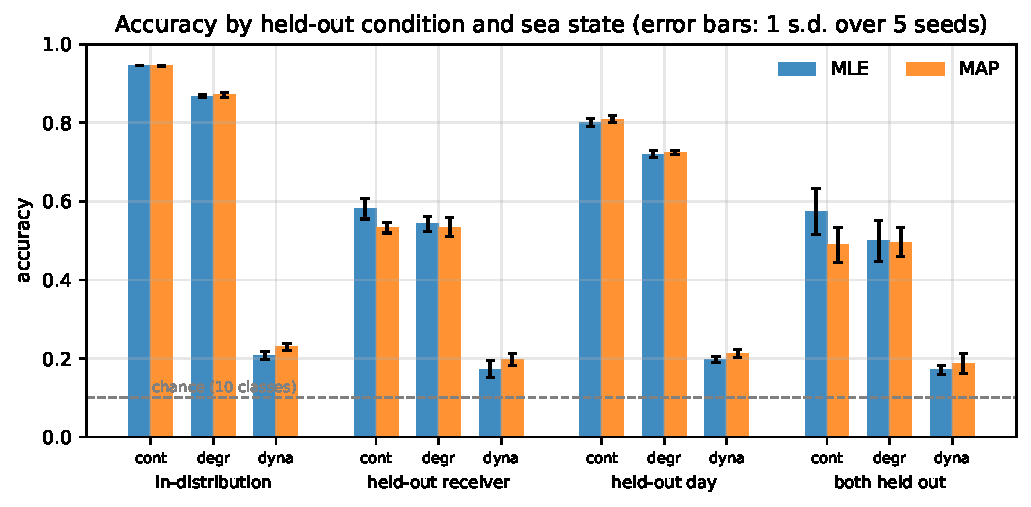
\includegraphics[width=\textwidth]{fig_accuracy_shift.pdf}
\caption{Accuracy by held-out condition and sea state. Error bars show one
standard deviation over five seeds. Each group of three bars is one test split
evaluated at the three tiers; \textsc{dynamic} was never seen in training.}
\label{fig:accuracy}
\end{figure}

\paragraph{Confidence does not degrade with it.}
The central result reported here is not the accuracy loss but the failure
of confidence to track it. Figure~\ref{fig:gap} plots mean predicted confidence
against accuracy for every cell; the shaded area is the discrepancy. On the
in-distribution split the two coincide almost exactly, giving an expected
calibration error of $0.007 \pm 0.001$ -- a model that, evaluated
conventionally, would appear entirely trustworthy. On the held-out receiver
accuracy falls to $0.581$ while mean confidence remains at $0.888$. On the
held-out sea state accuracy reaches $0.208$ while confidence stays at $0.572$:
the model is at chance and still asserting more than five times the certainty
that performance warrants. Expected calibration error rises from $0.007$ to
$0.382$, a fifty-fold degradation.

\begin{figure}[t]
\centering
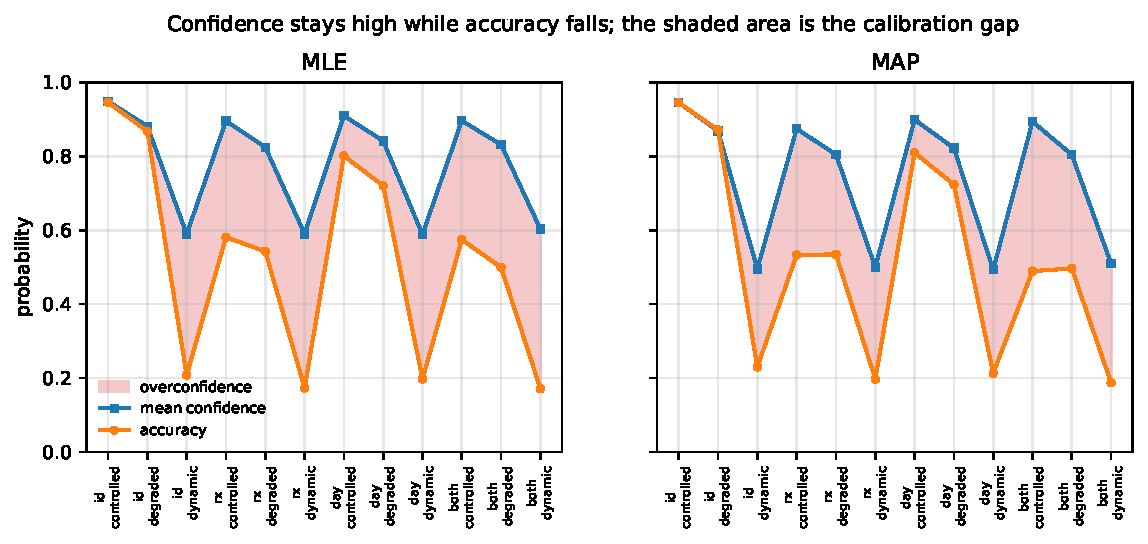
\includegraphics[width=\textwidth]{fig_confidence_gap.pdf}
\caption{Mean predicted confidence and accuracy for every evaluation cell. The
shaded region is the calibration gap. Confidence declines far more slowly than
accuracy as conditions become unfamiliar.}
\label{fig:gap}
\end{figure}

Figure~\ref{fig:reliability} presents the same finding as reliability diagrams.
In distribution the curve follows the diagonal closely. As conditions are
withheld it detaches and flattens, ending well below the diagonal: predictions
issued with high confidence are no more accurate than those issued with low
confidence.

\begin{figure}[t]
\centering
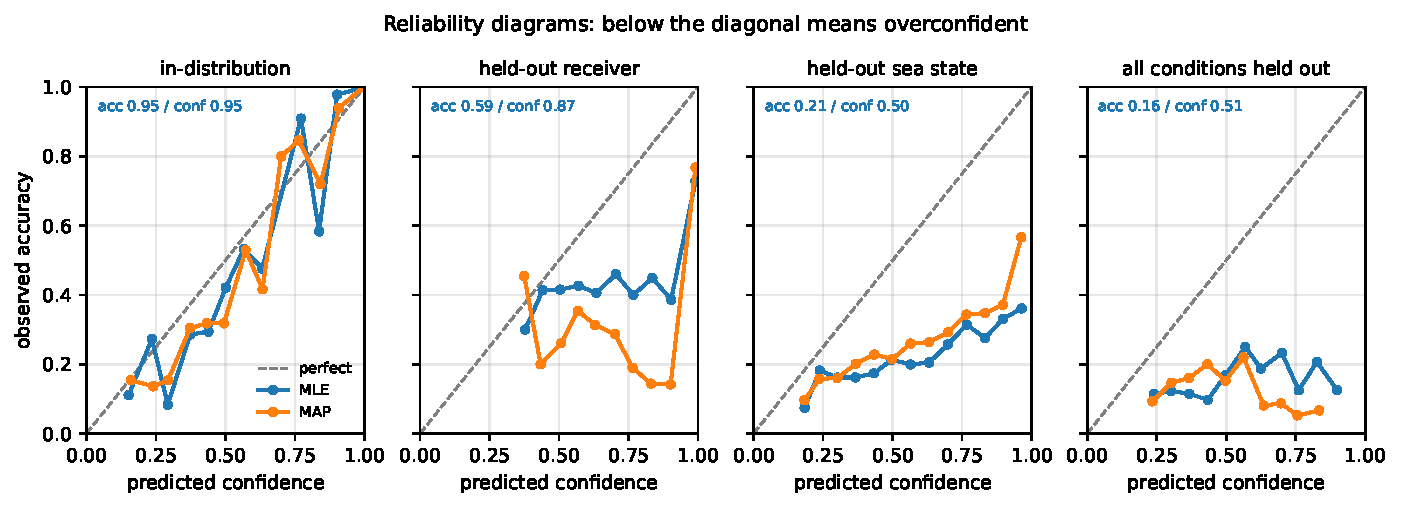
\includegraphics[width=\textwidth]{fig_reliability.pdf}
\caption{Reliability diagrams. A perfectly calibrated model traces the dashed
diagonal. Curves below it indicate overconfidence. Calibration is close to ideal
in distribution and deteriorates progressively as conditions absent from
training are introduced.}
\label{fig:reliability}
\end{figure}

\paragraph{The prior improves calibration, and improves its consistency more.}
MAP and MLE differ negligibly in accuracy: no cell shows a difference exceeding
twice the combined seed variation. Calibration is another matter. On the
withheld sea state MAP reduces expected calibration error by $0.116$, $0.114$,
$0.111$ and $0.109$ across the four test splits -- four independent measurements
agreeing to within $0.007$.

The more striking effect is on variability. At the \textsc{dynamic} tier the
standard deviation of MLE's calibration error across seeds is $0.062$, against
$0.025$ for MAP: the prior makes calibration roughly $2.4\times$ more
reproducible. No such effect appears at the two tiers seen during training
($0.9\times$ and $1.0\times$). Under distribution shift, then, the
point-estimate baseline is not merely overconfident but overconfident by an
amount that varies substantially with initialisation, and the prior stabilises
it. For an application in which a confidence value is intended to support an
operational decision, that unpredictability is arguably the more serious defect.

\paragraph{Overfitting was not the mechanism.}
Figure~\ref{fig:curves} shows the loss curves. Validation loss drifted only
$+0.001$ above its minimum by the final epoch for both objectives, and neither
model had clearly stopped improving at 80 epochs. The prior's benefit here
therefore did not arrive by preventing overfitting in the usual sense; dropout
at $p = 0.3$ appears to supply that regularisation already. The effect observed
is specifically on the confidence of predictions under distribution shift.

\begin{figure}[t]
\centering
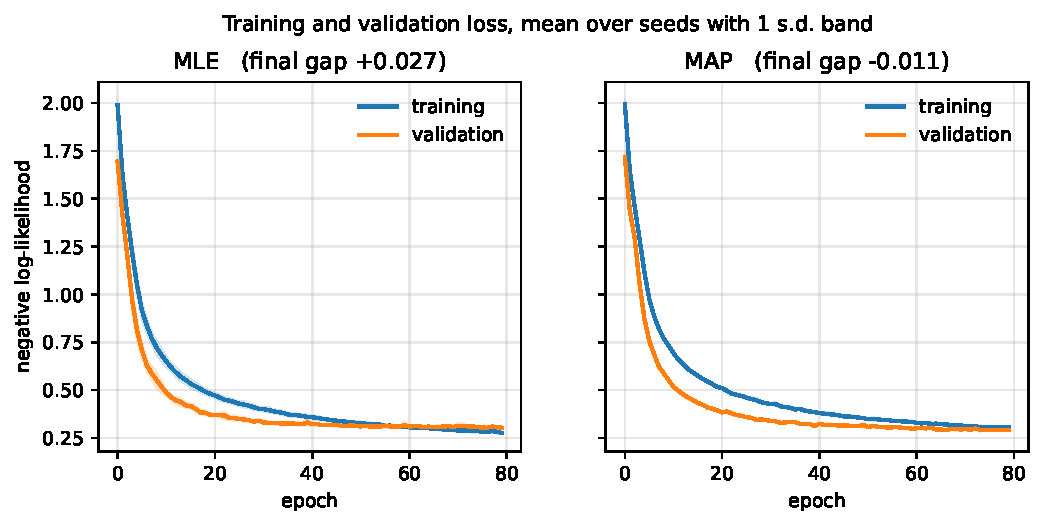
\includegraphics[width=\textwidth]{fig_loss_curves.pdf}
\caption{Training and validation negative log-likelihood, averaged over five
seeds with one standard deviation shaded. Neither objective shows pronounced
overfitting within the 80-epoch budget.}
\label{fig:curves}
\end{figure}

\paragraph{Phase information contributes.}
An ablation replaced the three-channel input with log magnitude alone, holding
everything else fixed. Under MLE the full representation was more accurate in
all twelve evaluation cells, with a median gain of $0.014$. No individual cell
exceeds twice its seed variation, but the probability of twelve independent
comparisons all favouring one condition by chance is $2^{-12}$, giving a
two-sided sign test $p = 0.0005$. The phase channels therefore contribute, even
though the per-cell differences are individually small. The corresponding
comparison under MAP is inconclusive (8 of 12 cells, $p = 0.39$).

\paragraph{Error structure.}
Figure~\ref{fig:confusion} shows confusion matrices in and out of distribution.
In distribution the matrix is close to diagonal. Under a held-out receiver
errors spread broadly rather than concentrating on particular emitter pairs,
which suggests the receiver change degrades the fingerprint representation
generally rather than making specific transmitters mutually confusable.

\begin{figure}[t]
\centering
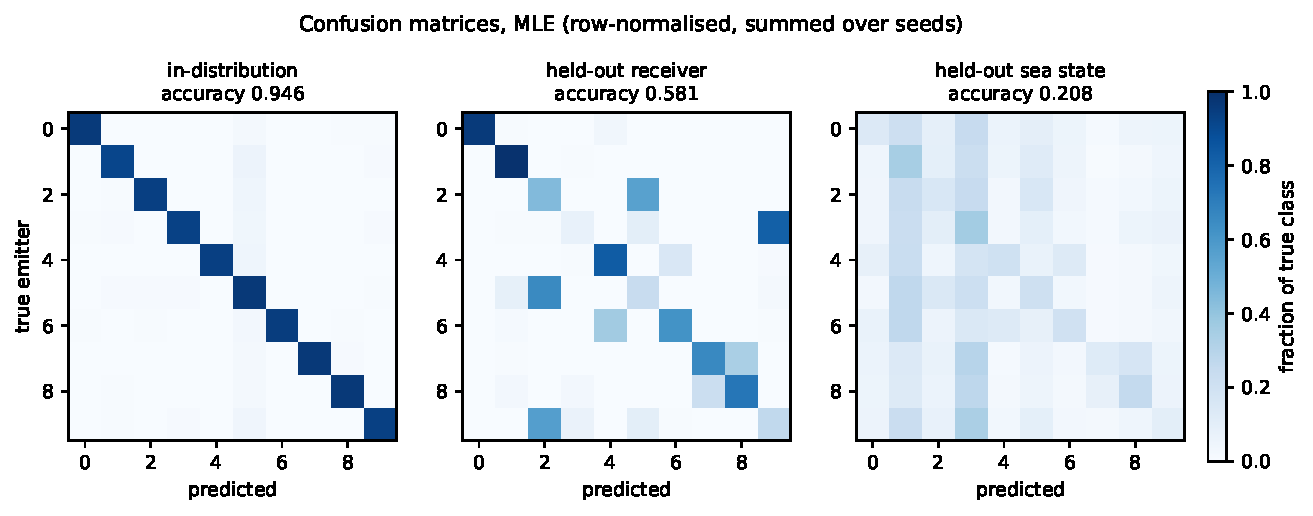
\includegraphics[width=\textwidth]{fig_confusion.pdf}
\caption{Row-normalised confusion matrices for the MLE model, summed over seeds.
Errors under distribution shift are broadly distributed rather than concentrated
in particular emitter pairs.}
\label{fig:confusion}
\end{figure}

\clearpage

\subsection{Approximate Bayesian results}
\label{sec:bayes-results}

The three variational methods of Section~\ref{sec:families} were trained under
the same architecture, data, optimiser and epoch budget as the point estimates,
across the same five seeds, and evaluated on the same twelve cells with $S = 20$
posterior samples per prediction. Table~\ref{tab:bayes-results} reports the full
grid; the discussion below draws on the two cells that bound it, the fully
in-distribution cell and the cell with the receiver, the capture day and the sea
state all held out.

\begin{table}[!htbp]
\centering
\caption{Accuracy and expected calibration error across every test split and sea-state tier, averaged over five seeds. The dynamic tier and the listed conditions were withheld from training. Seed-to-seed variation is omitted here for width and is shown as error bars in Figure~\ref{fig:ece-methods}.}
\label{tab:bayes-results}
\footnotesize
\begin{tabular}{llrrrrrr}
\toprule
Held out & Sea state & MLE & MAP & MC drop & Gauss VI & Conc $d{=}1$ & Conc $d{=}10$ \\
\midrule
\multicolumn{7}{l}{\emph{Accuracy}} \\
nothing held out & controlled & 0.946 & 0.945 & 0.945 & 0.941 & 0.944 & 0.948 \\
nothing held out & degraded & 0.867 & 0.871 & 0.872 & 0.851 & 0.854 & 0.841 \\
nothing held out & dynamic & 0.208 & 0.230 & 0.233 & 0.231 & 0.203 & 0.175 \\
receiver & controlled & 0.581 & 0.533 & 0.550 & 0.540 & 0.567 & 0.413 \\
receiver & degraded & 0.543 & 0.534 & 0.546 & 0.525 & 0.508 & 0.352 \\
receiver & dynamic & 0.173 & 0.197 & 0.187 & 0.193 & 0.170 & 0.126 \\
capture day & controlled & 0.801 & 0.810 & 0.805 & 0.802 & 0.787 & 0.770 \\
capture day & degraded & 0.720 & 0.724 & 0.726 & 0.709 & 0.691 & 0.637 \\
capture day & dynamic & 0.197 & 0.213 & 0.218 & 0.213 & 0.189 & 0.156 \\
receiver \& day & controlled & 0.574 & 0.489 & 0.510 & 0.479 & 0.520 & 0.416 \\
receiver \& day & degraded & 0.499 & 0.496 & 0.502 & 0.444 & 0.443 & 0.323 \\
receiver \& day & dynamic & 0.171 & 0.187 & 0.185 & 0.193 & 0.165 & 0.123 \\
\midrule
\multicolumn{7}{l}{\emph{Calibration error}} \\
nothing held out & controlled & 0.007 & 0.009 & 0.043 & 0.040 & 0.012 & 0.056 \\
nothing held out & degraded & 0.018 & 0.016 & 0.094 & 0.060 & 0.015 & 0.137 \\
nothing held out & dynamic & 0.382 & 0.265 & 0.170 & 0.190 & 0.369 & 0.169 \\
receiver & controlled & 0.315 & 0.342 & 0.222 & 0.268 & 0.263 & 0.237 \\
receiver & degraded & 0.282 & 0.270 & 0.144 & 0.211 & 0.274 & 0.201 \\
receiver & dynamic & 0.417 & 0.303 & 0.209 & 0.236 & 0.408 & 0.226 \\
capture day & controlled & 0.109 & 0.090 & 0.025 & 0.031 & 0.093 & 0.031 \\
capture day & degraded & 0.122 & 0.099 & 0.028 & 0.039 & 0.113 & 0.028 \\
capture day & dynamic & 0.391 & 0.280 & 0.182 & 0.205 & 0.383 & 0.188 \\
receiver \& day & controlled & 0.327 & 0.406 & 0.258 & 0.282 & 0.299 & 0.232 \\
receiver \& day & degraded & 0.333 & 0.309 & 0.187 & 0.289 & 0.331 & 0.217 \\
receiver \& day & dynamic & 0.432 & 0.323 & 0.221 & 0.236 & 0.421 & 0.227 \\
\bottomrule
\end{tabular}
\end{table}


\paragraph{Calibration improves and accuracy does not.}
Averaged over all twelve cells, expected calibration error falls from $0.261$
under MLE and $0.226$ under MAP to $0.149$ for fixed-rate dropout and $0.174$
for the Gaussian posterior. On the hardest cell the improvement is larger: MLE
reports mean confidence $0.603$ while classifying $17.1\%$ of bursts correctly,
for a calibration error of $0.432$; fixed-rate dropout reports $0.405$
confidence at $18.5\%$ accuracy, for $0.221$.

Accuracy is essentially unchanged. Every method sits between $16.5\%$ and
$19.3\%$ on that cell, against a chance floor of $10\%$, and no difference
approaches significance against the seed variation. This is the expected
outcome rather than a disappointment. Bayesian model averaging alters the shape
of the predictive distribution but rarely moves its peak, since the approximate
posterior is concentrated near the same solution the point estimate found. More
fundamentally, no inference procedure creates information: at $-5$ to $0$~dB
SNR with a $200$~ns delay spread the hardware fingerprint has been destroyed by
the channel, and a better posterior over weights cannot recover it. A large
accuracy gain here would be more suggestive of a leak between the training and
held-out conditions than of a genuine improvement.

The result being claimed is therefore narrower and more useful than an accuracy
gain. Holding accuracy fixed while confidence falls from $0.60$ to $0.41$ is
what makes the calibration comparison clean: the model has stopped asserting
competence it does not have.

\begin{figure}[t]
\centering
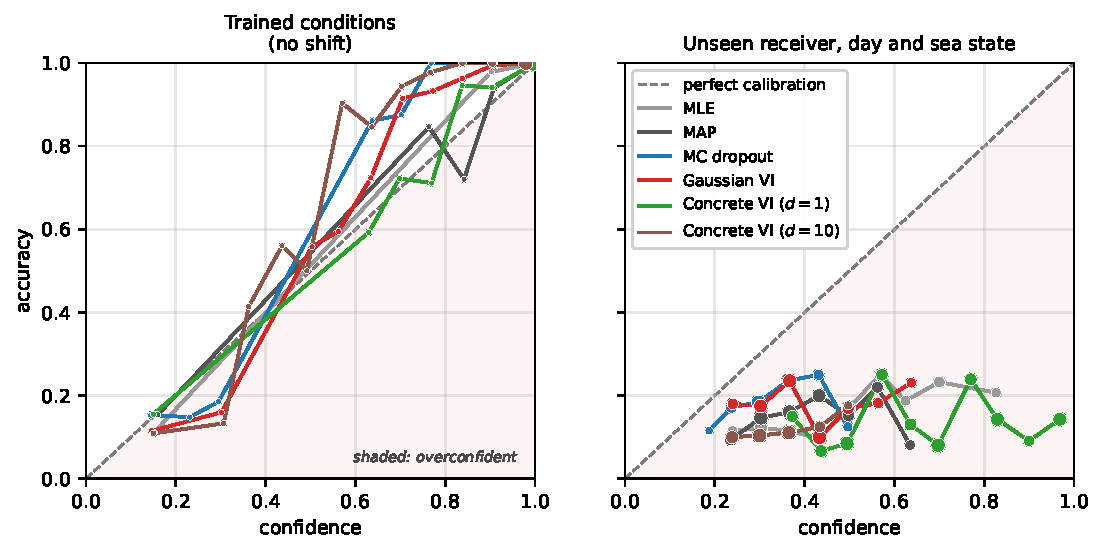
\includegraphics[width=\textwidth]{fig_reliability_bayes.pdf}
\caption{Reliability diagrams on trained conditions (left) and with the
receiver, capture day and sea state all held out (right). Marker area is
proportional to the number of predictions in each confidence bin, and bins
holding fewer than 25 predictions are omitted from the plot; the reported
calibration errors use every bin. On trained conditions the methods are hard to
separate. Under shift every curve falls into the shaded region, but the point
estimates and the learned-rate posterior extend furthest to the right, still
issuing high-confidence predictions at close to chance accuracy.}
\label{fig:reliability-bayes}
\end{figure}

\begin{figure}[t]
\centering
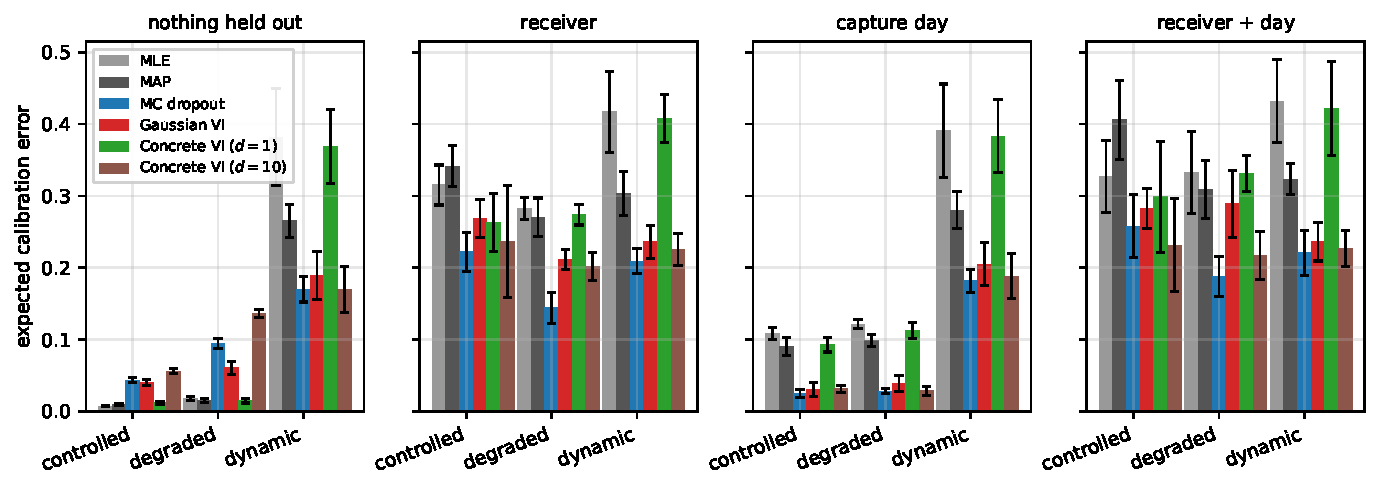
\includegraphics[width=\textwidth]{fig_ece_methods.pdf}
\caption{Expected calibration error for all five methods across every test split
and sea-state tier, with one seed standard deviation. Bars whose intervals
overlap are not treated as different in the text.}
\label{fig:ece-methods}
\end{figure}

\paragraph{Uncertainty rises where it should.}
Table~\ref{tab:uncertainty} and Figure~\ref{fig:uncertainty-split} give the
decomposition of Eq.~\eqref{eq:decomposition}. Total predictive entropy rises by
a factor of $5.4$ to $6.8$ between the trained cell and the fully held-out one,
approaching the ceiling of $\log K = 2.303$ that represents complete ignorance.
Epistemic uncertainty rises by a factor of $4.5$ for fixed-rate dropout, $6.4$
for the Gaussian posterior and $12.1$ for the learned-rate posterior. The point
estimates cannot appear in this comparison at all: with a single weight vector
the epistemic term is identically zero for every input, however unfamiliar, as
noted in Section~\ref{sec:decomposition}.

The split between the two components is itself informative, and reading only the
epistemic term would give a misleading picture. Under the most severe corruption
the aleatoric term dominates, reaching $1.30$ nats for fixed-rate dropout
against $0.34$ epistemic. Every sampled model converges on a near-uniform
prediction, so they \emph{agree} that the burst cannot be identified, and mutual
information is low precisely because the disagreement has gone. That is the
correct description of what has happened. The signal has been destroyed, which
is aleatoric, rather than merely being unfamiliar to a model that could
otherwise classify it.

\begin{figure}[t]
\centering
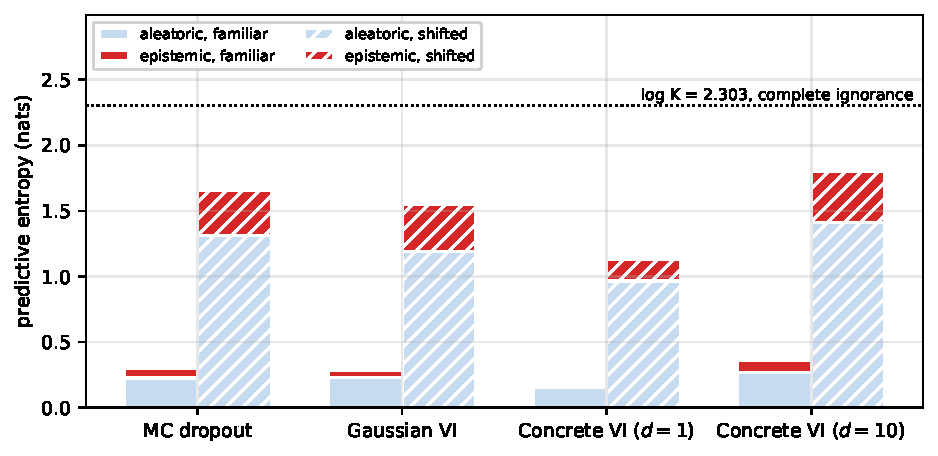
\includegraphics[width=0.85\textwidth]{fig_uncertainty_split.pdf}
\caption{Predictive entropy split into aleatoric and epistemic components on
trained conditions and on the fully held-out cell. Stacked height is total
entropy, bounded above by $\log K = 2.303$. Under severe corruption the
aleatoric component dominates: the sampled models agree that the burst cannot be
identified.}
\label{fig:uncertainty-split}
\end{figure}

\begin{table}[!htbp]
\centering
\caption{Predictive entropy split into aleatoric and epistemic parts, on trained conditions and on the fully held-out cell. The point estimates are absent because a single set of weights has no epistemic term to measure.}
\label{tab:uncertainty}
\small
\begin{tabular}{llrrrr}
\toprule
Method & Conditions & Total & Aleatoric & Epistemic & Wrong / right \\
\midrule
MC dropout & trained & 0.302 & 0.226 & 0.076 & 2.15 \\
MC dropout & held out & 1.654 & 1.310 & 0.344 & 1.02 \\
\addlinespace
Gaussian VI & trained & 0.285 & 0.229 & 0.056 & 3.09 \\
Gaussian VI & held out & 1.547 & 1.193 & 0.353 & 1.05 \\
\addlinespace
Concrete VI ($d{=}1$) & trained & 0.165 & 0.151 & 0.013 & 5.90 \\
Concrete VI ($d{=}1$) & held out & 1.127 & 0.965 & 0.162 & 1.02 \\
\addlinespace
Concrete VI ($d{=}10$) & trained & 0.357 & 0.269 & 0.088 & 2.00 \\
Concrete VI ($d{=}10$) & held out & 1.804 & 1.409 & 0.396 & 0.99 \\
\bottomrule
\end{tabular}
\end{table}


\paragraph{The fitted dropout rate reports the regulariser, not the data.}
At the regulariser strength specified by the method, $d = 1/N$, the fitted rates
collapse. Across five independent seeds they follow the same per-layer pattern,
approximately $0.006$ at the first convolution, $0.10$ at the second, $0.012$ at
the third and $0.006$ before the classifier, and the reproducibility rules out
an initialisation artefact. On trained conditions this is the best-calibrated
method of the five, at $0.012$ against $0.007$ for MLE. Under shift it is the
worst, at $0.421$ against MLE's $0.432$, and significantly worse than fixed-rate
dropout in 8 of the 12 cells. A rate near zero is very nearly a point estimate,
so the method reverts to exactly the failure it was meant to remove.

The obvious reading is that the data has judged a stochastic posterior
unnecessary, the training distribution containing no Dynamic-tier bursts and no
unseen receiver. That reading is wrong, and the reason is worth following,
because it concerns a term that is easy to overlook.

Only one part of the objective resists $p \to 0$. Written out, the divergence in
Eq.~\eqref{eq:vi-loss} for a dropout posterior has two competing pieces,
\begin{equation}
\operatorname{KL}\big[q_\phi \,\|\, p\big]
= \underbrace{w\,\frac{\lVert M \rVert_2^2}{1-p}}_{\text{rises with } p}
\; + \;
\underbrace{d \cdot D \cdot \big[\, p\log p + (1-p)\log(1-p) \,\big]}_{\text{Bernoulli entropy, minimised at } p = 0.5},
\label{eq:concrete-kl}
\end{equation}
where $D$ is the number of inputs to the layer. The entropy term is the only
thing pushing the rate up, and its coefficient is $dD$. With $d = 1/N$ that
coefficient is $D/N$, so how much uncertainty a layer is permitted to retain
depends on how many inputs it happens to have. For this network the coefficient
ranges from $0.022$ before the classifier to $0.172$ before the second
convolution, and the second convolution is precisely the one layer that kept a
usable rate. The per-layer pattern tracks the strength of the regulariser, not
any property of the layers.

Table~\ref{tab:dropout-sweep} tests this directly by scaling $d$. At $d = 10$
the collapse disappears and the rates settle at $0.319$, $0.449$, $0.343$ and
$0.147$ with seed standard deviations below $0.01$. Calibration on the hardest
cell improves from $0.421$ to $0.227$, statistically indistinguishable from
fixed-rate dropout's $0.221$, and mean calibration error over all twelve cells
falls from $0.248$ to $0.163$. The method is not broken; its default
regularisation is too weak.

Pushing further exposes the opposite failure. At $d = 50$ and $d = 100$ the
rates converge on $0.5$, which is simply where Bernoulli entropy is largest. In
the single-seed sweep of Table~\ref{tab:dropout-sweep} the spread across layers
falls from $0.316$ at $d=10$ to $0.059$ at $d=100$: the regulariser has
overwhelmed the likelihood and is reporting its own optimum rather than
distinguishing the layers. The fitted rate is
informative only in a middle band, and locating that band requires a sweep over
$d$. Concrete Dropout was introduced to remove the need to choose
$p_{\text{drop}}$ by hand, and on this problem it replaces that choice with a
choice of $d$ that is no easier to make and has a failure mode at each end.

One cost is not recovered by any setting. Mean accuracy at $d = 10$ is $0.440$
against roughly $0.52$ for every other method, concentrated in the held-out
receiver cells. Correcting the regulariser buys calibration and pays for it in
accuracy, which fixed-rate dropout did not have to do.

\begin{table}[!htbp]
\centering
\caption{Effect of the entropy regulariser scale on Concrete Dropout (seed 0). The fitted rates collapse towards $0$ when the term is weak and saturate at the Bernoulli entropy maximum of $0.5$ when it is strong; the spread across layers, which measures how far the data still distinguishes them, is largest in between. Calibration improves monotonically while accuracy falls.}
\label{tab:dropout-sweep}
\small
\begin{tabular}{rrrrrl}
\toprule
Scale & Mean $p$ & Spread & Mean accuracy & Mean ECE & Fitted rates \\
\midrule
1 & 0.032 & 0.105 & 0.501 & 0.270 & 0.00, 0.11, 0.01, 0.00 \\
10 & 0.304 & 0.316 & 0.438 & 0.175 & 0.31, 0.44, 0.33, 0.13 \\
50 & 0.450 & 0.104 & 0.384 & 0.180 & 0.45, 0.49, 0.47, 0.39 \\
100 & 0.472 & 0.059 & 0.401 & 0.150 & 0.47, 0.50, 0.48, 0.44 \\
\bottomrule
\end{tabular}
\end{table}


\begin{figure}[t]
\centering
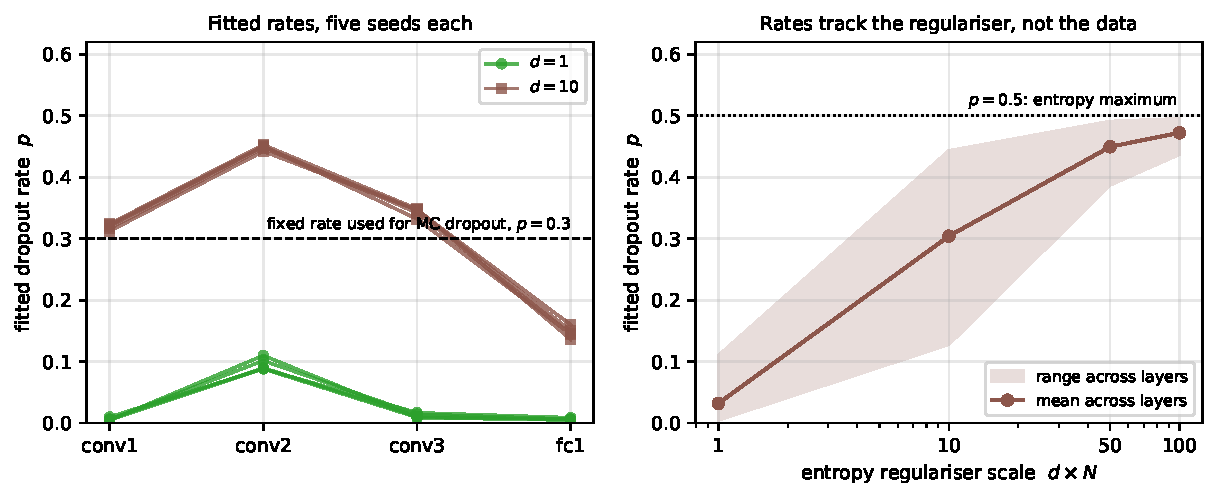
\includegraphics[width=0.7\textwidth]{fig_dropout_rates.pdf}
\caption{Left: dropout rates fitted at the default regulariser strength
($d=1$) and at the corrected one ($d=10$), one line per seed. The per-layer
\emph{shape} is identical at both strengths and across all ten runs, so the data
does express a consistent preference between layers; what the regulariser sets
is the \emph{level}. Right: mean fitted rate against regulariser scale, shaded
by the range across layers. Weak regularisation collapses every rate to zero,
strong regularisation saturates them at the Bernoulli entropy maximum of $0.5$,
and the layers are distinguished from one another only in between.}
\label{fig:dropout-rates}
\end{figure}

\paragraph{Posterior width identifies which layers the data constrains.}
The Gaussian posterior offers a diagnostic the other two do not. Against a prior
standard deviation of $\sigma_p = 0.374$, the fitted posterior standard
deviations settle at roughly $0.02$ for the first convolution and $0.23$ to
$0.31$ for the first fully connected layer (Figure~\ref{fig:posterior-sigma}).
A layer whose posterior remains far below the prior has been pinned down by the
data; one that drifts up towards the prior has not, and is falling back on the
prior because the likelihood has little to say about those weights. The first
fully connected layer holds $63\%$ of the network's parameters and is largely
unidentified, which suggests the architecture is not capacity-limited, and is
consistent with the observation that accuracy did not improve.

This figure also serves as the collapse check for the variational runs. Had
every layer risen to meet the prior, the KL term would have overwhelmed the
likelihood and the network would have learned nothing, which is a known failure
mode of variational inference under a wide prior. It did not occur here.

\begin{figure}[t]
\centering
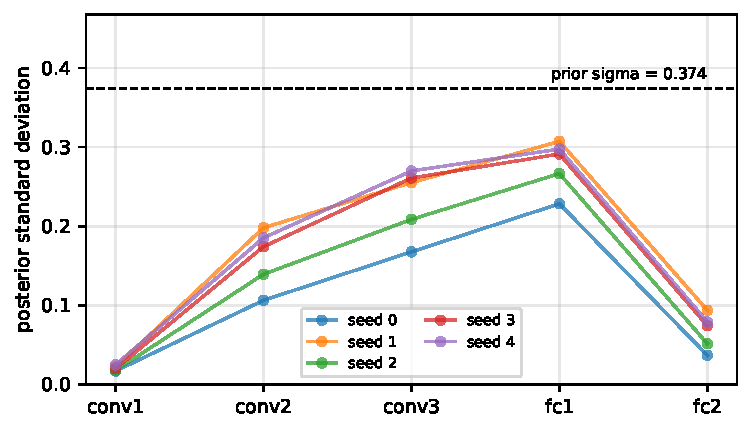
\includegraphics[width=0.7\textwidth]{fig_posterior_sigma.pdf}
\caption{Fitted posterior standard deviation per layer for the Gaussian
variational posterior, one line per seed, against the prior standard deviation
implied by the MAP penalty. Early convolutional layers are strongly constrained
by the data; the first fully connected layer is close to the prior.}
\label{fig:posterior-sigma}
\end{figure}

\paragraph{Identification against signal-to-noise ratio.}
Table~\ref{tab:poi} reports probability of identification by sea-state tier,
holding the receiver and capture day familiar so that channel severity is the
only quantity varying. Identification is essentially unaffected between the
Controlled and Degraded tiers, falling only from $0.946$ to $0.867$ under MLE
across a $10$~dB reduction in signal-to-noise ratio. It then collapses to
$0.208$ on the Dynamic tier. The fingerprint survives moderate degradation and
does not survive severe degradation, and the transition is abrupt rather than
gradual.

Resolution here is limited by a choice made in the data pipeline: the
signal-to-noise ratio drawn for each individual burst is applied and then
discarded rather than stored, so identification can be reported against a tier
whose range is known but not against the exact ratio of a given burst.
Recording the per-burst draws would permit a continuous curve and is a small
change to make.

\begin{table}[!htbp]
\centering
\caption{Probability of identification by sea-state tier, with the signal-to-noise range each tier spans. The receiver and capture day are familiar throughout, so severity is the only quantity varying down the table. Chance is $0.100$ for ten emitters. The Dynamic tier was withheld from training.}
\label{tab:poi}
\footnotesize
\begin{tabular}{llrrrrrr}
\toprule
Sea state & SNR (dB) & MLE & MAP & MC drop & Gauss VI & Conc $d{=}1$ & Conc $d{=}10$ \\
\midrule
controlled & $+15$ to $+25$ & 0.946 & 0.945 & 0.945 & 0.941 & 0.944 & 0.948 \\
degraded & $+5$ to $+15$ & 0.867 & 0.871 & 0.872 & 0.851 & 0.854 & 0.841 \\
dynamic$^{\dagger}$ & $-5$ to $0$ & 0.208 & 0.230 & 0.233 & 0.231 & 0.203 & 0.175 \\
\bottomrule
\end{tabular}
\\[2pt]\footnotesize $^{\dagger}$withheld from training.
\end{table}


\paragraph{What the representation looks like.}
The accuracy tables establish that identification fails under shift but not why,
and two different mechanisms would produce the same number. The fingerprint may
still be present while the network's representation of it has moved, or the
fingerprint may no longer be present at all. These correspond exactly to the
epistemic and aleatoric terms of Eq.~\eqref{eq:decomposition}, so distinguishing
them matters for interpreting every calibration result above.

Figure~\ref{fig:embedding} projects the $128$-unit activation of the first fully
connected layer, the network's internal description of a burst immediately
before classification. To keep the comparison honest, a separability statistic
is computed in the full $128$ dimensions rather than in the projection: the
fraction of bursts whose nearest neighbour in embedding space carries the same
emitter label, which is $1.0$ for perfect separation and $0.1$ at chance for ten
emitters. The projection is for viewing; the statistic is what the claim rests
on.

\begin{figure}[t]
\centering
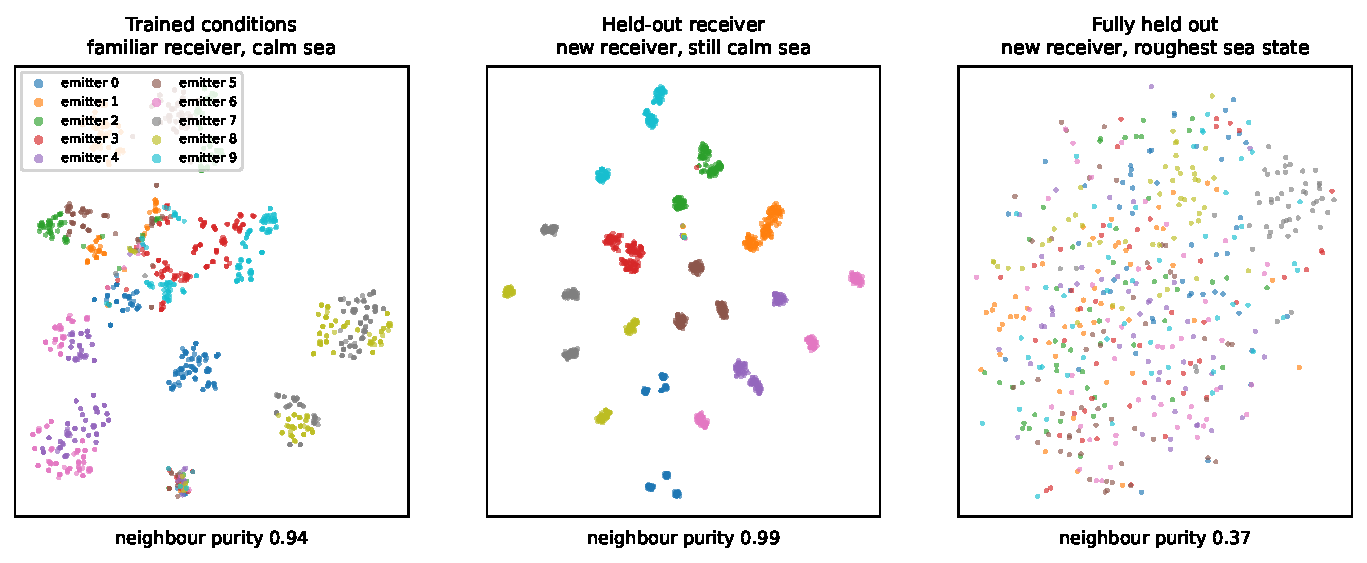
\includegraphics[width=\textwidth]{fig_embedding.pdf}
\caption{t-SNE projection of the $128$-unit penultimate representation, coloured
by emitter, with neighbour purity computed in the full embedding space rather
than in the projection. Chance purity is $0.100$. The middle panel is the
informative one: the emitters are more cleanly separated than on trained data
($0.993$) while accuracy has fallen to $0.550$, so the fingerprint survives the
receiver change and the decision boundaries do not. In the right-hand panel the
structure itself is largely gone.}
\label{fig:embedding}
\end{figure}

\paragraph{What the uncertainty does not do.}
One limitation should be recorded plainly, because it bounds the operational
claim. Within a single evaluation cell, epistemic uncertainty barely separates
correct predictions from incorrect ones: the ratio of mean epistemic uncertainty
on wrong predictions to that on right ones is $1.02$ to $1.05$ for all three
methods (Table~\ref{tab:uncertainty}). The methods detect that conditions as a
whole have moved away from those they were trained on, and they lower their
confidence accordingly. They do not reliably indicate \emph{which} individual
bursts within a degraded batch have been misattributed. Distribution-level
warning is a weaker guarantee than per-prediction triage, and a system built on
these results should be designed around the former.

% Flush any figures still queued, so that floats cannot spill past the
% Discussion section and into the bibliography.
\clearpage

%======================================================================
\section{Discussion}
%======================================================================

The question posed in Section~\ref{sec:bayes} was not whether a network can
identify a transmitter, which the literature had already settled, but whether it
knows when it cannot. The answer, across five seeds and twelve evaluation cells,
is that a point estimate does not and a variational posterior partially does.

The point-estimate result is the sharper of the two. A classifier reaching
$94.6\%$ accuracy with a calibration error of $0.007$ on familiar conditions
falls to $17.1\%$ accuracy, barely above the $10\%$ chance floor, on a sea state
it never trained on, while still reporting $60\%$ mean confidence. By any
evaluation confined to the training distribution it looks reliable. The failure
is silent, and it is silent in the specific way that matters operationally: the
model does not become visibly confused, it remains confident and becomes wrong.

Replacing the point estimate with an approximate posterior does not repair the
accuracy, and Section~\ref{sec:bayes-results} argued that it should not be
expected to. What changes is the honesty of the reported confidence. Mean
calibration error falls by $43\%$ relative to MLE, and on the hardest cell the
model's stated confidence drops from $0.60$ to $0.41$ while its accuracy stays
where it was. For a physical-layer attribution system this is the difference
that carries operational weight. A track attributed with $60\%$ confidence and
wrong $83\%$ of the time will be acted upon; the same track at $41\%$ confidence
is escalated to an operator. The classification is equally wrong in both cases.
Only one of them is defensible.

Three findings qualify that conclusion.

First, the choice of posterior family matters less than having one at all. The
Gaussian and fixed-rate dropout posteriors differ significantly in only 4 of 24
comparisons, despite representing quite different distributions over weights,
one continuous and factorised over every weight, the other a discrete mask over
units. The gap between either of them and the MAP point estimate is much the
larger effect.

Second, the improvement is not uniform, and on trained conditions it reverses.
Both methods are \emph{worse} calibrated than MLE in the fully in-distribution
cell, $0.043$ and $0.040$ against $0.007$, because they add uncertainty
everywhere, including where the point estimate was already correct to be
confident. Averaged calibration error conceals this. A deployment that expects
to operate mostly within its training distribution would be paying a real cost
for insurance against a case that rarely arrives, and the trade is only clearly
favourable when unfamiliar conditions are the operational norm, which for a
maritime emitter-identification system they are.

Third, and least expected, the method that learns its own dropout rate does not
remove the hyper-parameter it was designed to remove. At its default setting the
fitted rates collapse to near zero and calibration under shift is no better than
maximum likelihood. Strengthening the entropy term by a factor of ten restores
the rates and brings calibration level with fixed-rate dropout; strengthening it
further pins every rate at the entropy maximum, where the fitted value describes
the regulariser rather than the data. What began as a choice of $p_{\text{drop}}$
becomes a choice of $d$, with a distinct failure mode at each extreme and no
principled way to locate the middle except to sweep.

This is the most transferable finding here, and it generalises past dropout. The
quantity governing how much uncertainty a variational method expresses is itself
set by a coefficient in the objective. When that coefficient is left at a
default whose magnitude depends on architecture, as $d \cdot D$ does on layer
width, the resulting uncertainty is an accident of network shape. It is worth
checking, for any method advertised as learning its own uncertainty, which term
opposes the collapse and whether it is strong enough to do so.

\paragraph{Why identification fails, and why that distinction matters.}
The embedding analysis separates two explanations that the accuracy tables
cannot, and the result is sharper than expected. On trained conditions the
penultimate representation resolves the ten emitters into distinct
neighbourhoods, with neighbour purity $0.941$ against accuracy $0.945$: the
representation separates the emitters and the decision boundaries agree with it.

Holding the sea state calm and changing only the receiver, purity rises to
$0.993$ while accuracy falls to $0.550$. The fingerprint is not merely still
present, it is more cleanly separated than on the data the network trained on,
and the classifier is nonetheless wrong on nearly half the bursts. Whatever has
broken is not the representation. The information required to identify the
emitter survives the receiver change essentially intact, and what has moved is
the mapping from that representation to a label. This is epistemic failure in
the precise sense the decomposition intends: the evidence is recoverable, and
something as small as re-fitting the final layer on a handful of labelled bursts
from the new receiver would plausibly recover most of the lost accuracy.

One caveat belongs with that comparison. The held-out receiver split contains
bursts from a single receiver, whereas the in-distribution split spans the
seventeen used in training, so part of the tighter clustering is reduced
within-class variance rather than a genuinely better representation. The gap
between purity and accuracy is measured within one split and is unaffected by
this, but the $0.941$ against $0.993$ comparison across splits should not be
read as the receiver change improving anything.

Adding the Dynamic tier changes the character of the failure. Purity falls to
$0.366$, well above the chance value of $0.100$ but far below either of the
other two panels, and accuracy falls to $0.185$. Here the representation itself
has been degraded, so no decision rule applied to it could recover the emitter
for most bursts. That is a statement about the signal rather than the model, and
it is aleatoric.

The uncertainty decomposition, computed independently of any of this, agrees.
Relative to trained conditions, the receiver change multiplies epistemic
uncertainty by $3.31$ and aleatoric by only $1.48$, so the larger movement is in
the term that tracks the model. The Dynamic tier reverses the ordering,
multiplying epistemic by $4.52$ and aleatoric by $5.79$: the larger movement is
now in the term that tracks the signal. Two measurements that share no
machinery, one a nearest-neighbour statistic on the penultimate layer and the
other a mutual information computed from sampled predictions, identify the same
two failure modes and assign them the same way round.

This is the same division that Eq.~\eqref{eq:decomposition} makes numerically,
arrived at independently, and the agreement is what licenses the interpretation
offered above. It also accounts for a pattern in the decomposition that is
easily misread. Epistemic uncertainty rises monotonically with channel
severity, from $0.076$ to $0.176$ to $0.317$ nats for fixed-rate dropout across
the three tiers, which is the expected behaviour. Its \emph{share} of total
uncertainty does not: it peaks at the middle tier and falls at the most severe
one, $0.252$ to $0.277$ to $0.192$, and the same inversion appears in all three
methods.

That peak is where the fingerprint is partly present and partly destroyed, so
the sampled models genuinely disagree about what they are seeing. At the most
severe tier they stop disagreeing, because there is nothing left to disagree
about, and the uncertainty they report is correctly attributed to the signal
rather than to the weights. A reader tracking only the epistemic share would
read that fall as the method failing at exactly the point it is most needed.
It is the opposite: the decomposition is reporting, accurately, that the
failure has changed character.

\paragraph{Returning to the claimed contribution.}
Section~\ref{sec:bayes} argued that the reviewed literature treats channel and
receiver robustness on one hand and uncertainty quantification on the other as
largely separate concerns, and that the combination was the gap this work would
occupy. That claim survives the results, and the reason is visible in the
numbers rather than merely asserted. The robustness literature would have
reported the accuracy column of Table~\ref{tab:bayes-results} and concluded that
the problem is hard under shift. The uncertainty-quantification literature would
have reported the calibration column on in-distribution data and concluded that
these methods are well calibrated, which on the evidence of the $0.007$ to
$0.043$ range in the top rows is defensible. Only holding both axes at once
produces the finding that actually matters operationally: the methods are
calibrated where they are not needed and the point estimates fail precisely
where they are, and the two facts are invisible to an evaluation that fixes
either axis.

The same combination is what makes the learned-rate result legible. Concrete
Dropout is reported in the uncertainty literature as an improvement, and on
in-distribution data measured here it is exactly that at its default setting,
the best calibrated of the five. It is only when a held-out sea state is
introduced that the method inverts, and only when the regulariser is swept that
the reason becomes visible. A study holding either axis fixed would have
recorded a confident conclusion about this method, and which conclusion it
recorded would have depended on which axis it fixed.

\paragraph{What this means for the decision the system supports.}
Section~\ref{sec:bayes} claimed that a physical-layer attribution decision needs
a calibrated confidence rather than an arg-max label, because the confidence is
what an analyst acts on. The results give that claim a magnitude. On the hardest
cell the point estimate and the Bayesian posterior return the same wrong
emitter, and the accuracy difference between them is not significant. What
differs is the number attached: $0.60$ against $0.41$, on a prediction that is
wrong $83\%$ of the time. Whether that track is acted on or escalated turns
entirely on the quantity this work measures, and not at all on the quantity a
conventional evaluation would have reported.

\paragraph{Limitations.}
The maritime channel is simulated. The transmitter fingerprints and receiver
imperfections in the WiSig captures are real hardware, but no public dataset
provides maritime captures with known emitter labels, so the propagation model
is applied to recordings made indoors at $2.462$~GHz. The tier definitions are
physically motivated but not validated against sea trials, and the mapping from
sea state to Rician $K$-factor and delay spread is a modelling choice. The
cohort is ten emitters drawn from the 150 available; behaviour at operational
population sizes is untested. The evaluation withholds one receiver and one
capture day, which measures sensitivity to those factors but does not establish
how the model behaves across the full diversity of either. Identification is
reported against sea-state tier rather than as a continuous function of
signal-to-noise ratio, because the pipeline discards the per-burst value it
draws; each tier spans a known range, so this is a loss of resolution rather
than of correctness, but it is a loss.

Two limitations are inherited from modelling choices rather than from the data.
The mean-field posterior assumes every weight is independent, which they are
not, and this is known to make variational inference underestimate posterior
spread; it is a candidate explanation for why the Gaussian posterior did not
outperform the simpler dropout one. And the softmax likelihood assumes a closed
set: probability is distributed across the ten known emitters and must sum to
one, so an eleventh transmitter would necessarily be assigned to one of the ten.
A deployed system faces an open set, and nothing measured here speaks to that
case.

Most importantly, as Section~\ref{sec:bayes-results} recorded, the uncertainty
produced here is informative at the level of a distribution and close to
uninformative at the level of an individual prediction.

\paragraph{Further work.}
The most direct extension is per-prediction reliability, since that is where the
present methods are weakest. Deep ensembles are the obvious comparison, being
usually better calibrated than single-mode variational methods and known to
separate correct from incorrect predictions more effectively, at a training cost
this project could not afford. A second direction follows from the negative
result on learned rates: fitting uncertainty parameters against a small
held-out sample of shifted data, rather than against the training distribution,
would test directly whether the failure identified here is a property of the
objective or of the data it was optimised over.

A third follows directly from the embedding result and is cheap to run. If the
representation separates emitters at purity $0.993$ on a receiver the network
never trained on, while the classifier reaches only $0.550$, then the loss is in
the final mapping rather than in the features. Re-fitting only the last layer on
a small number of labelled bursts from the new receiver, with the convolutional
stack frozen, would establish how much of that gap is recoverable and at what
labelling cost. A large recovery would show that receiver-induced failure is an
adaptation problem rather than a sensing one, which is an operationally
different and much cheaper thing to fix.

Two extensions were identified in Section~\ref{sec:bayes} as motivating the
Bayesian treatment and are now supported by it without having been attempted.
Continual learning, adding emitters over time without retraining from scratch,
requires the current posterior to serve as the prior for the next increment,
which a point estimate cannot provide and the methods here can. Active learning
requires a ranking of what the model does not yet know, in order to prioritise
which conditions or emitters to collect. The epistemic term supplies that
ranking, though the limitation above applies directly: it ranks conditions
reliably and individual bursts poorly, so it would support deciding which sea
states to go and record rather than which specific captures to label.

Finally, the caveat entered in Section~\ref{sec:bayes} stands unchanged. The
captures are $2.462$~GHz WiFi preambles, not maritime-band transmissions, so
what this work demonstrates is the evaluation framework and the behaviour of
these methods within it. Transfer to operational waveforms and frequencies
remains untested, and the quantity most likely to change is the severity at
which the fingerprint disappears, not the finding that confidence outlasts
accuracy when it does.

%======================================================================
\section{Conclusion}
%======================================================================

A convolutional classifier trained to identify ten physical transmitters reaches
$94.6\%$ accuracy on the conditions it was trained on, with a calibration error
of $0.007$. Evaluated on a sea state it has never seen, it falls to $17.1\%$,
against a chance floor of $10\%$, and reports $60\%$ confidence while doing so.
Any evaluation confined to the training distribution would have certified this
model as reliable.

Replacing the single set of weights with an approximate posterior leaves the
accuracy where it is. That is the correct outcome rather than a shortfall: at
the signal-to-noise ratios of the withheld tier the hardware fingerprint has
been destroyed by the channel, and the embedding analysis confirms it directly.
What changes is the confidence attached to the answer, which falls from $0.60$
to $0.41$ on the hardest condition and improves calibration by $43\%$ on
average. For a system whose output an operator must decide whether to act on,
that is the quantity that matters, and it is invisible to an accuracy-only
evaluation.

Three results qualify that. The particular family assumed for the posterior
matters far less than assuming one at all; the improvement reverses on
in-distribution data, where the added uncertainty is unnecessary; and the method
that learns its own dropout rate does not remove the hyper-parameter it was
meant to remove. On that last point, the fitted rate collapses to zero at the
default regulariser strength and saturates at the entropy maximum when the
regulariser is strong, so it is informative only within a band that has to be
located by sweeping. The general lesson is that the uncertainty a variational
method expresses is set by a coefficient in its objective, and when that
coefficient carries a default whose magnitude depends on layer width, the
uncertainty reported is partly an accident of architecture.

The evaluation framework is the durable contribution. The captures are WiFi
preambles and the maritime channel is simulated, so the specific numbers should
not be read as operational performance. What transfers is the finding that
confidence outlasts accuracy under distribution shift, that the gap is
measurable, and that the measurement is cheap enough to run on any emitter
identification system before it is fielded.

\clearpage
\bibliographystyle{plainnat}
\bibliography{bibliography}

\end{document}
